\documentclass[11pt]{article}
\pdftrailerid{}
\pdfsuppressptexinfo=15
\pdfgentounicode=1
\pdfglyphtounicode{tfm:lmsy10/mapsto}{007C}
\pdfglyphtounicode{tfm:lmex10/parenleftbig}{0028}
\pdfglyphtounicode{tfm:lmex10/parenrightbig}{0029}
\pdfglyphtounicode{tfm:lmex10/bracketleftbig}{005B}
\pdfglyphtounicode{tfm:lmex10/bracketrightbig}{005D}
\pdfglyphtounicode{tfm:lmex10/floorleftbig}{230A}
\pdfglyphtounicode{tfm:lmex10/floorrightbig}{230B}
\pdfglyphtounicode{tfm:lmex10/ceilingleftbig}{2308}
\pdfglyphtounicode{tfm:lmex10/ceilingrightbig}{2309}
\pdfglyphtounicode{tfm:lmex10/vextendsingle}{23D0}
\pdfglyphtounicode{tfm:lmex10/parenleftbigg}{0028}
\pdfglyphtounicode{tfm:lmex10/parenrightbigg}{0029}
\pdfglyphtounicode{tfm:lmex10/floorleftbigg}{230A}
\pdfglyphtounicode{tfm:lmex10/floorrightbigg}{230B}
\pdfglyphtounicode{tfm:lmex10/braceleftbigg}{007B}
\pdfglyphtounicode{tfm:lmex10/bracerightbigg}{007D}
\pdfglyphtounicode{tfm:lmex10/parenleftBigg}{0028}
\pdfglyphtounicode{tfm:lmex10/parenrightBigg}{0029}
\pdfglyphtounicode{tfm:lmex10/bracketleftBigg}{005B}
\pdfglyphtounicode{tfm:lmex10/bracketrightBigg}{005D}
\pdfglyphtounicode{tfm:lmex10/braceleftBigg}{007B}
\pdfglyphtounicode{tfm:lmex10/bracketlefttp}{23A1}
\pdfglyphtounicode{tfm:lmex10/bracketrighttp}{23A4}
\pdfglyphtounicode{tfm:lmex10/bracketleftbt}{23A3}
\pdfglyphtounicode{tfm:lmex10/bracketrightbt}{23A6}
\pdfglyphtounicode{tfm:lmex10/bracelefttp}{23A7}
\pdfglyphtounicode{tfm:lmex10/braceleftbt}{23A9}
\pdfglyphtounicode{tfm:lmex10/braceleftmid}{23A8}
\pdfglyphtounicode{tfm:lmex10/braceex}{23AA}
\pdfglyphtounicode{tfm:lmex10/circlemultiplydisplay}{2A02}
\pdfglyphtounicode{tfm:lmex10/summationtext}{2211}
\pdfglyphtounicode{tfm:lmex10/producttext}{220F}
\pdfglyphtounicode{tfm:lmex10/summationdisplay}{2211}
\pdfglyphtounicode{tfm:lmex10/productdisplay}{220F}
\pdfglyphtounicode{tfm:lmex10/integraldisplay}{222B}
\pdfglyphtounicode{tfm:lmex10/hatwide}{0302}
\pdfglyphtounicode{tfm:lmex10/floorleftBig}{230A}
\pdfglyphtounicode{tfm:lmex10/floorrightBig}{230B}
\pdfglyphtounicode{tfm:lmex10/ceilingleftBig}{2308}
\pdfglyphtounicode{tfm:lmex10/ceilingrightBig}{2309}
\pdfglyphtounicode{tfm:lmex10/radicalBigg}{221A}
\usepackage[T1]{fontenc}
\usepackage{lmodern}
\usepackage{microtype}
\usepackage[margin=1.05in]{geometry}
\usepackage{amsmath,amssymb,amsthm,mathtools}
\usepackage{enumitem,booktabs,array}
\usepackage{tikz}
\usetikzlibrary{arrows.meta,positioning,calc,decorations.pathreplacing}
\usepackage[numbers,sort&compress]{natbib}
\usepackage[colorlinks=true,linkcolor=blue!55!black,citecolor=blue!55!black,urlcolor=blue!55!black]{hyperref}
\usepackage[nameinlink,noabbrev,capitalise]{cleveref}

\newtheorem{theorem}{Theorem}[section]
\newtheorem{lemma}[theorem]{Lemma}
\newtheorem{proposition}[theorem]{Proposition}
\newtheorem{corollary}[theorem]{Corollary}
\theoremstyle{definition}
\newtheorem{definition}[theorem]{Definition}
\theoremstyle{remark}
\newtheorem{remark}[theorem]{Remark}

\AddToHook{env/theorem/begin}{\crefalias{theorem}{theorem}}
\AddToHook{env/lemma/begin}{\crefalias{theorem}{lemma}}
\AddToHook{env/proposition/begin}{\crefalias{theorem}{proposition}}
\AddToHook{env/corollary/begin}{\crefalias{theorem}{corollary}}
\AddToHook{env/definition/begin}{\crefalias{theorem}{definition}}
\AddToHook{env/remark/begin}{\crefalias{theorem}{remark}}

\newcommand{\E}{\mathbb E}
\newcommand{\Prb}{\mathbb P}
\DeclareMathOperator{\Var}{Var}
\DeclareMathOperator{\Cov}{Cov}
\DeclareMathOperator{\TV}{TV}
\DeclareMathOperator{\supp}{supp}
\DeclareMathOperator{\poly}{poly}
\newcommand{\one}{\mathbf 1}
\newcommand{\calM}{\mathcal M}
\newcommand{\calE}{\mathcal E}
\newcommand{\calT}{\mathcal T}
\newcommand{\wt}{\operatorname{wt}}
\newcommand{\R}{\mathbb R}
\newcommand{\N}{\mathbb N}
\newcommand{\abs}[1]{\left|#1\right|}
\newcommand{\norm}[1]{\left\lVert#1\right\rVert}
\newcommand{\set}[1]{\left\{#1\right\}}
\newcommand{\eps}{\varepsilon}
\newcommand{\ceil}[1]{\left\lceil#1\right\rceil}
\newcommand{\floor}[1]{\left\lfloor#1\right\rfloor}
\newcommand{\dd}{\,\mathrm d}
\newcommand{\bit}{\operatorname{bit}}
\newcommand{\PM}{\operatorname{PM}}

\setlist{topsep=4pt,itemsep=3pt,parsep=0pt}
\renewcommand{\labelitemi}{\(\bullet\)}
\numberwithin{equation}{section}
\hypersetup{pdftitle={A Fully Polynomial Randomized Approximation Scheme for Perfect Matchings in General Graphs},pdfauthor={OpenAI}}
\title{A Fully Polynomial Randomized Approximation Scheme\\
for Perfect Matchings in General Graphs}
\author{OpenAI}
\date{September 23, 2026}
\begin{document}
\maketitle
\begin{abstract}
We give a fully polynomial randomized approximation scheme (FPRAS) for
counting perfect matchings in arbitrary finite simple undirected graphs,
resolving the general-graph perfect-matching approximation problem.
The algorithm returns zero with certainty when no perfect matching exists.
Otherwise, it achieves relative error $\eps$ with failure probability at
most $\delta$ in worst-case bit time polynomial in the input length,
$\eps^{-1}$, and $\log\delta^{-1}$.
\end{abstract}
\tableofcontents
\section{Introduction}
\label{sec:introduction}

Let $G=(V,E)$ be a finite simple undirected graph. A perfect matching is a
set of edges incident to each vertex exactly once. Write
\[
 Z(G)=\#\{M\subseteq E:M\text{ is a perfect matching of }G\}.
\]
A fully polynomial randomized approximation scheme approximates $Z(G)$
within a prescribed relative error, with a prescribed success probability,
in time polynomial in the input length and the reciprocal error.
The confidence parameter enters through its logarithm. We prove the
following theorem, including a bound on the time of every execution.

\begin{theorem}\label{thm:main}
There is a uniform classical randomized algorithm which, given $G$ and
rational parameters $0<\eps<1$ and $0<\delta<1/2$, returns a nonnegative
rational number $\widehat Z$ such that
\[
 \Prb\bigl[(1-\eps)Z(G)\le \widehat Z\le(1+\eps)Z(G)\bigr]
 \ge 1-\delta.
\]
If $Z(G)=0$, the output is zero with certainty. The worst-case bit running
time is polynomial in the input encoding length, $\eps^{-1}$, and
$\log\delta^{-1}$.
\end{theorem}

As consequences, \cref{sec:prescribed-degree} gives counting schemes for
edge subsets with prescribed vertex degrees and for matchings of a
specified size. On feasible inputs, its samplers always return a
feasible object and approximate the corresponding uniform law in total
variation.

\subsection{History and significance}
Perfect matchings illustrate the distinction between finding a
combinatorial structure and counting its realizations. Edmonds gave a
polynomial-time algorithm for finding a maximum matching in a general
graph~\cite{Edmonds1965}. Valiant proved that exact counting is
\#P-complete even for bipartite graphs, where it is the permanent of a
zero--one matrix~\cite{Valiant1979}. Pfaffian methods give
polynomial-time exact counting for planar graphs~\cite{Kasteleyn1963}.

For approximation, three problems must be distinguished: counting all
matchings, counting bipartite perfect matchings, and counting perfect
matchings in general graphs. Jerrum and Sinclair gave an FPRAS for the
total number of matchings in an arbitrary graph, summed over all
cardinalities~\cite[Corollary~4.5]{JerrumSinclair1989}.
Their perfect-matching algorithm applied when the ratio of near-perfect
matchings, which leave exactly two vertices unmatched, to perfect
matchings was bounded by a fixed polynomial~\cite[Theorem~5.3]{JerrumSinclair1989}.
Without such a bound, perfect matchings can carry too little stationary
mass for this sampling approach. Approximating the total number of
matchings therefore does not isolate its perfect-matching contribution
with relative accuracy.

Jerrum, Sinclair, and Vigoda removed the ratio restriction in the
bipartite setting and obtained an FPRAS for the permanent of every
nonnegative matrix~\cite[Theorem~1.1]{JerrumSinclairVigoda2004}.
Their method assigns weights to near-perfect states according to their
two unmatched vertices and learns suitable weights while gradually
changing edge activities. The general-graph question was explicitly
raised by Jerrum and Sinclair~\cite[Section~7(i)]{JerrumSinclair1989}
and remained a benchmark for approximate counting. Cai and Liu relate
it to approximation for the eight-vertex model~\cite{CaiLiu2020};
Fei, Goldberg, and Lu distinguish the spin-system parameter line
equivalent to general perfect-matching approximation from the region
covered by their FPRAS~\cite[Proposition~1.2 and Theorem~1.5]{FeiGoldbergLu2025}.
\Cref{thm:main} answers the general-graph perfect-matching approximation
problem affirmatively.

A direct extension of the bipartite chain faces a precise obstruction.
\v{S}tefankovi\v{c}, Vigoda, and Wilmes constructed graphs on which every
JSV-type chain has either exponentially small stationary probability
of perfect matchings or exponentially slow mixing, even with arbitrary
weights depending on the hole pattern~\cite[Definition~2.1 and
Theorem~2.2 in the full version]{StefankovicVigodaWilmes2018}.
Here JSV type means the perfect-and-near-perfect state space with the
specified Broder proposals and a Metropolis acceptance rule. The
sampler below uses a different state space: a product of
perfect-matching spaces on an enlarged colored graph, with exchanges
of alternating cycles between coordinates. Its energy comparison is
proved for these states and moves.

Subsequent permanent algorithms sharpen the bipartite result.
Bez\'{a}kov\'{a}, \v{S}tefankovi\v{c}, Vazirani, and Vigoda accelerated the
cooling schedule and improved the analysis of the matching
chain~\cite{BezakovaStefankovicVaziraniVigoda2008}.
Chen, Vigoda, and Yang obtain a further improvement through restricted
Poincar\'e inequalities and coupled flows~\cite{ChenVigodaYang2026};
Chen, Guo, Vigoda, and Yang develop an energy-weighted
multicommodity-flow comparison and improve the running time
again~\cite{ChenGuoVigodaYang2026}. These results concern bipartite
perfect matchings.

For nonbipartite graphs, Yi gives deterministic relative approximation
for hafnians, the weighted sums over perfect matchings, when the
$n$-vertex support has minimum degree at least $(1/2+\gamma)n$ and
nonzero weights lie in $[\theta,1]$~\cite[Theorem~1.1]{Yi2026}.
Here $0<\gamma<1/2$ and $0<\theta\le1$ are fixed constants, and the
polynomial running-time exponent may depend on them.
\Cref{thm:main} has no density promise on its simple unweighted input.

The proof below also builds on the methodological framework of weighted
matching chains. Alternating overlays and weight-preserving switches
underlie the encodings of Jerrum and Sinclair and of Jerrum, Sinclair,
and Vigoda~\cite{JerrumSinclair1989,JerrumSinclairVigoda2004}.
Their sampling-to-counting strategy learns local partition ratios while
gradually changing activities.
Here these ratios are exposed by marked edges in an enlarged graph,
and vertex scaling maintains a row-wise balance condition. The
capacity bound, subdivision and marked-edge identities needed for this
construction are proved explicitly.

Energy comparison through weighted demands has classical antecedents
in multicommodity-flow bounds for mixing~\cite{Sinclair1992}.
Our comparison differs from routing every demand along a path of chain
transitions: long-arc conversions enter a signed identity and need not
be legal single updates. The resulting estimate initially controls
only additive functions of two matching coordinates. The separate
product-space argument is essential to obtain a spectral gap for
arbitrary functions. It uses the classical orthogonal decomposition
into coordinate interactions~\cite[Section~2]{EfronStein1981}; the
ordered assignment of residual terms and the replication estimate are
proved below.

\subsection{Proof architecture}

The counting algorithm starts with the complete graph, whose perfect
matchings are easy to count, and gradually suppresses the nonedges of
$G$ by decreasing their positive activities. It estimates the ratios
of successive partition functions and multiplies them. To keep the
observations statistically useful, it updates vertex scales from
estimates of the two-hole partition ratios: partition functions after
deleting two vertices, divided by the current partition function.
Accurate estimates keep each row maximum between two absolute
constants. A vertex scale
multiplies every complete matching weight by the same factor, preserving
the probability law used to estimate the current counting ratio.

The purpose of balance is to control the extra mass introduced by an
auxiliary graph. We replace each logical edge by a weighted path, with
a bijection between logical perfect matchings and matchings using only
these real path edges. We then add weak clique edges in overlapping
bags indexed by a tree. Under balance, the added edges increase the
partition function by at most a factor of two, so a sample uses only
real edges with probability at least one half. A specially marked
auxiliary edge exposes the corresponding two-hole partition ratio.
These are exact event identities; they provide both the counting
estimate and the data for the next scale update.

To prove the inflation bound, \cref{thm:logical-hole-bound} assigns a
pairing capacity to each even hole set using the strongest bottleneck
paths between its vertices. The capacity pays for the weights of
possible added edges on those holes. Subdivision transfers this bound
to the real graph while making incident effective strengths comparable.
The resulting geometry supplies the tree of clique bags. Thus the
hole estimates control the probability of the observable events,
while the tree-bag structure supplies a sampler for their law.

That sampler uses local switches in one matching and exchanges
alternating cycles between two matching coordinates. Its energy
comparison initially controls only additive functions of the two
coordinates. A quadrangulation adapted to the bag labels gives an exact
signed identity for a whole-cycle difference
(\cref{lem:quadrangulation,thm:pair-energy}). The identity is not a
route through chain transitions: long arc conversions may change many
edges. Two-matching encodings instead compare its terms with local
switches and cycle exchanges, with polynomially bounded multiplicity.

A ladder of nearby weight distributions then places many independent
coordinates at each tier. An ordered orthogonal decomposition ensures
that each coordinate-interaction term is charged to at most one pair.
Replication reduces the coefficient of their combined contribution
enough to absorb it. This yields a spectral gap for
arbitrary functions of the product state (\cref{lem:replica-gap}).
The bottom tier has unit activities and admits exact counting and
ideal sampling by a tree dynamic program. The sampler requires no
balance assumption. It therefore remains defined, with the same time
bound, after an inaccurate empirical estimate; balance is used only
to prove that accurate estimates propagate through the counting stages.

\Cref{tab:graph-laws} summarizes the changes of law. Finally,
\cref{sec:counting,sec:complexity} account for all arithmetic and
finite-bit random choices. Every polynomial has an absolute degree;
the constants are chosen for transparent estimates rather than
practical efficiency.

\begin{table}[ht]
\centering
\small
\begin{tabular}{@{}p{.18\textwidth}cp{.61\textwidth}@{}}
\toprule
Object & Vertices & Relation of matching laws \\
\midrule
Input $G$ & $n$ & The target is its unweighted count $Z(G)$. \\
Complete graph & $n$ & Raw activities $w^{(j)}$ gradually suppress the nonedges of $G$. \\
Vertex scaling & $n$ & Activities $\lambda$ preserve the normalized raw matching law. \\
Real paths & $N$ & Subdivision gives a matching bijection with a common weight multiplier. \\
Colored bags & $N$ & Their activities $W$ recover the real law when every sampled edge is revealed as real. \\
Weight tiers & $N$ & Common-interval clamps of $W$ connect the unit-activity law to the bag law on one colored state space. \\
\bottomrule
\end{tabular}
\caption{The successive graphs and probability laws. Here $n$ is the
original vertex count and $N$ the enlarged count. Scaling, subdivision,
conditioning, and clamping have distinct roles.}
\label{tab:graph-laws}
\end{table}

The specialized combinatorial and sampling arguments are proved here.
We use Edmonds's algorithm for the initial matching-existence test
and Hoeffding's bounded-variable inequality for concentration and
confidence amplification~\cite{Edmonds1965,Hoeffding1963}.
\section{Preliminaries}
\label{sec:preliminaries}

Logarithms are natural unless a base is indicated.

\subsection{Weighted matchings and holes}
We allow parallel edges distinguished by colors. A matching specifies
the actual colored edges it uses. For positive rational activities
$a=(a_e)$, put
\[
 \wt_a(M)=\prod_{e\in M}a_e,\qquad
 Z_a(-U)=\sum_{M\in\calM(H-U)}\wt_a(M),
 \qquad Z_a=Z_a(-\varnothing),
\]
where $H$ is the underlying graph and $\calM(H-U)$ is its set of perfect
matchings after deleting $U$. The empty graph has one perfect matching,
of weight one. Whenever $Z_a>0$, define
\[
 g_a(U)=\frac{Z_a(-U)}{Z_a},\qquad
 \pi_a(M)=\frac{\wt_a(M)}{Z_a}.
\]
These weighted colored graphs are intermediate spaces constructed from
the simple input graph. Their representation is explicit: vertices,
colored edges, and rational activities are stored individually. The
main theorem retains the finite simple undirected input model; it does
not assert a counting algorithm for compressed edge multiplicities or
for singleton-covering loops.

We call the vertices in $U$ \emph{holes}. For distinct vertices we abbreviate
$g_a(\{i_1,\ldots,i_k\})$ to $g_a(i_1\cdots i_k)$.
Collapsing parallel activities into their
sum preserves every partition function. Conditional on a collapsed
edge, its original type can be recovered with probabilities
proportional to the summands.

The union of two matchings, with common edges retained twice, has
maximum degree two. Its nontrivial components are alternating paths
and even alternating cycles. Swapping the layers along a component
preserves the product of their weights. In the union of two perfect
matchings, deleting common identical edges leaves disjoint alternating
cycles; different colors on the same pair of vertices form a cycle
of length two. We fix a vertex order and a color order once and for
all. They resolve every combinatorial tie in the proof.

\subsection{Bottleneck similarities}
For a positive weighted connected graph define
\begin{equation}\label{eq:bottleneck}
 B_{ij}=\max\left\{1,\ \max_{P:i\leadsto j}\ \min_{e\in P}a_e\right\}
 \quad (i\ne j).
\end{equation}
Simple paths suffice. This symmetric similarity satisfies
$B_{ij}\ge\min\{B_{ik},B_{kj}\}$: concatenating two paths and erasing
loops cannot lower their minimum activity. For $t>1$, its equivalence
classes are the connected components of the graph retaining edges of
activity at least $t$. Singletons are included. At $t=1$ we take one
class containing every vertex, consistently with the floor at one.
For an even set $U$ define its \emph{pairing capacity}
\begin{equation}\label{eq:pairing-capacity}
 \Phi_B(U)=\max_{\mathcal P}\prod_{ij\in\mathcal P}B_{ij},
 \qquad \Phi_B(\varnothing)=1,
\end{equation}
where $\mathcal P$ runs over pairings of $U$. We use this quantity only
in proofs; the counting algorithm never needs to enumerate pairings
or compute $\Phi_B(U)$ for a general hole set.

\subsection{Tree bags}
\begin{definition}\label{def:tree-bags}
A \emph{tree-bag graph} consists of a finite rooted tree of labels and
a finite even vertex set. A label $l$ at level $k$ has height $h_l=2^k$;
the root has level zero and a child has level one greater than its
parent. Each vertex belongs to either one label or two adjacent
labels. The bag at $l$ is the set of vertices belonging to $l$.
For each unordered pair of distinct vertices and each common label
$l$, there is one edge of color $l$. There are no other edges.
For an integer parameter $D\ge1$, its reference activities obey
\begin{equation}\label{eq:bag-weight-range}
 \frac{h_l}{D}\le W_{xy,l}\le3h_l.
\end{equation}
We also consider activities obtained by clamping all $W_e$ to one
common interval $[a,b]\subset(0,\infty)$.
\end{definition}

Every vertex pair has at most two edge colors. At any bag, the
interfaces with its parent and its different children are disjoint:
a vertex in two such interfaces would have at least three memberships.
Empty bags and repeated underlying vertex sets are permitted.
Clamping is monotone and does not increase the ratio of a larger
activity to a smaller one. In particular, reference activities of
nearby labels remain comparable after clamping.

\subsection{Dirichlet energy and approximation}
For a finite reversible Markov kernel $P$ with stationary law $\mu$,
its Dirichlet energy is
\begin{equation}\label{eq:dirichlet}
 \calE_{\mu,P}(f)
 =\frac12\sum_{x,y}\mu(x)P(x,y)(f(x)-f(y))^2.
\end{equation}
A Poincar\'e inequality $\Var_\mu f\le\gamma^{-1}\calE_{\mu,P}(f)$
means that the spectral gap is at least $\gamma$. A symmetric proposal
$Q$ has Metropolis acceptance probability~\cite{MetropolisEtAl1953,Hastings1970} $\min\{1,\mu(y)/\mu(x)\}$
for a proposed move from $x$ to $y$. Its off-diagonal stationary capacity is
\begin{equation}\label{eq:metropolis-capacity}
 \mu(x)P(x,y)=Q(x,y)\min\{\mu(x),\mu(y)\}.
\end{equation}
We regard inapplicable proposals as holding moves. All state spaces
used below contain at least one perfect matching; thus their positive
activities define probability laws with full support on that space.

Total variation is
$\|\mu-\rho\|_{\TV}=\frac12\sum_x|\mu(x)-\rho(x)|$.
A deterministic map, or a common randomized postprocessing kernel,
does not increase total variation, by the triangle inequality.
Two finite laws at total variation distance $\eta$ admit a coupling
that disagrees with probability $\eta$: first match the common masses
$\min(\mu(x),\rho(x))$, then couple the remainders. Applying this
construction successively bounds the discrepancy probability of an
adaptive simulation by the sum of its conditional one-step errors.
\section{Controlling the cost of unmatched vertices}
\label{sec:holes}

This section proves the bound that will control the additional edges in
our sampling graph.  It uses only alternating paths and differentiation
of a finite partition function.

Let $V$ have even cardinality $n\ge2$, and give every edge of the complete
logical graph $K_V$ a positive activity $\lambda_{ij}$. Use the weighted
matching notation of \cref{sec:preliminaries}, abbreviating
$\calM(K_V-U)$ to $\mathcal M(-U)$. For any positive activity array $a$
on this graph, define the row maxima
\[
 r_i(a)=\max_{j\ne i}g_a(ij).
\]
The activities $a$ are \emph{balanced} if $1/4\le r_i(a)\le1$ for
every $i$. Let $B$ be the bottleneck similarity of $\lambda$ from
\eqref{eq:bottleneck}, and let $\Phi_B$ be its pairing capacity from
\eqref{eq:pairing-capacity}.

The estimate we need controls every even hole set, although balance
only bounds the two-hole ratios:

\begin{theorem}[Logical hole bound]
\label{thm:logical-hole-bound}
Let $\lambda$ be balanced, let $B$ be its bottleneck similarity, and set
\[
 D_0=10^8(n+1)^4.
\]
For every even set $U\subseteq V$,
\begin{equation}
\label{eq:logical-hole-bound}
 g_\lambda(U)\Phi_B(U)\le 2D_0^{|U|/2}.
\end{equation}
\end{theorem}

To prove this, we will add a small activity proportional to $B_{ij}$
on every pair. Bounds for two and four holes keep the resulting
partition inflation below two. Any pairing of an arbitrary hole set
can then be inserted using the added edges, giving the stated bound.

We use two elementary alternating-path comparisons. Such weight-preserving
overlays also underlie the weighted matching encodings in
\cite{JerrumSinclair1989,JerrumSinclairVigoda2004}; the comparisons and
their constants needed here are proved below. In an overlay of
two matchings, edges retain their layer.  Common edges can be kept as
two parallel copies.  A path starting at a vertex unmatched in exactly
one layer is then uniquely determined, and switching its edges between
the layers preserves the product of their weights.

\begin{lemma}[Four-hole inequality]
\label{lem:four-holes}
For any positive activities $\mu$ and four distinct vertices $a,b,c,d$,
\[
 g_\mu(abcd)\le
 g_\mu(ab)g_\mu(cd)+g_\mu(ac)g_\mu(bd)
                         +g_\mu(ad)g_\mu(bc).
\]
Consequently, if every row maximum is at most $4$, then
\begin{equation}
\label{eq:small-hole-bounds}
 g_\mu(\varnothing)=1,\qquad
 g_\mu(U)\le4\quad(|U|=2),\qquad
 g_\mu(U)\le48\quad(|U|=4).
\end{equation}
\end{lemma}

\begin{proof}
Overlay $M\in\mathcal M(-\{a,b,c,d\})$ and
$P\in\mathcal M(-\varnothing)$.  The alternating path from $a$ ends at
one of $b,c,d$, say $b$.  Switch that path between the layers.  The
output layers miss $\{c,d\}$ and $\{a,b\}$, respectively, and their
product weight is unchanged.  This map is injective for the specified
endpoint $b$: in the output overlay, follow the path from $a$ and switch
it back.  The same argument applies to endpoints $c,d$.
Summing the three injective comparisons and dividing by $Z_\mu^2$
proves the inequality.  The remaining assertions follow immediately.
\end{proof}

The four-hole comparison controls small hole sets by row maxima. We
next need an additional factor when two holes are joined by a strong
path. Normalizing by the row maximum at the moving hole will make
the successive relocation errors add, without multiplying along the
path.

The next lemma is stated with $\mu\ge\lambda$ so that it continues to
apply while we add activities to the graph.  Its bottleneck similarity
always remains the one defined from $\lambda$.

\begin{lemma}[Relocating a hole along a strong path]
\label{lem:hole-relocation}
Let $B$ be defined by \eqref{eq:bottleneck}, and suppose that
$\mu_e\ge\lambda_e$ for every edge and
\[
 \frac18\le r_i(\mu)\le4\qquad(i\in V).
\]
If $|U|\in\{2,4\}$ and $i,j\in U$ are distinct, then
\begin{equation}
\label{eq:hole-relocation-bound}
 g_\mu(U)\le\frac{10^5n}{B_{ij}}.
\end{equation}
\end{lemma}

\begin{proof}
Throughout this proof, omit the subscript $\mu$ from $g$ and $r$.
Write $B=B_{ij}$.  For $B\le8$, the assertion follows from
\eqref{eq:small-hole-bounds}.  Suppose therefore that $B>8$, and choose
a simple path from $i$ to $j$ whose $\lambda$-activities, and hence its
$\mu$-activities, are all at least $B$.

We first give one step of the relocation.  Let $a$ be the hole currently
on this path, let $S$ be the current hole set, and let $z$ be the next
vertex.  Thus $a\in S$ and $\mu_{az}\ge B$.
If $z\in S$, inserting $az$ in a matching missing $S$ is injective and
increases its weight by $\mu_{az}$.  Hence
\begin{equation}
\label{eq:adjacent-hole-fill}
 \frac{g(S)}{r_a}\le
 \frac{g(S\setminus\{a,z\})}{B r_a}\le\frac{32}{B}.
\end{equation}
The last inequality uses $|S|\le4$, \eqref{eq:small-hole-bounds}, and
$r_a\ge1/8$.

Now suppose $z\notin S$.  Choose $p\ne z$ with $g(zp)=r_z$.
Inserting $az$ gives $g(az)\le1/\mu_{az}\le1/B<1/8$, so $p\ne a$.
Overlay $M\in\mathcal M(-S)$ and $P\in\mathcal M(-\{z,p\})$.
The path from $a$ starts with an edge of $P$.  Its endpoint belongs to
exactly one of the following three cases.
\begin{enumerate}[label=\textup{(\roman*)},leftmargin=*]
\item It ends at $z$.  Switching the path gives layers missing
$S\setminus\{a\}\cup\{z\}$ and $\{a,p\}$.
The product weight is unchanged.
\item It ends at $p$, which requires $p\notin S$.
Switching gives layers missing $S\setminus\{a\}\cup\{p\}$ and
$\{a,z\}$.  Insert $az$ in the second layer, making it perfect.
The product weight increases by $\mu_{az}\ge B$.
\item It ends at $x\in S\setminus\{a,p\}$.
Switching gives layers missing $S\setminus\{a,x\}$ and
$\{z,p,a,x\}$.  Insert $az$ in the second layer; its remaining holes
are $\{p,x\}$.  Again the product weight increases by at least $B$.
\end{enumerate}
These cases exhaust the possibilities.  Indeed, the degree-one
vertices in the overlay are exactly the symmetric difference of the
two hole sets; if $p\in S$, then $p$ is isolated and cannot be an
endpoint of the path.

The edge $az$ is absent from both input layers, since the first misses
$a$ and the second misses $z$. Switching cannot create an edge absent
from the overlay. Each map is injective when its case and endpoint are specified.
For case (i), the inverse switches the output path from $a$.
For cases (ii) and (iii), first remove the inserted edge $az$ from the
second output layer, then switch the path from $a$ in the resulting
overlay.  This reconstructs both input layers, including their common
edges.  Summing over all inputs, using $g(ap)\le r_a$, and dividing by
$Z_\mu^2r_z$ yields
\begin{equation}
\label{eq:relocation-step}
\begin{split}
 g(S)\le{}&\frac{r_a}{r_z}
                g(S\setminus\{a\}\cup\{z\})\\
 &+\frac{1}{B r_z}\left[
   \mathbf 1_{\{p\notin S\}}g(S\setminus\{a\}\cup\{p\})
   +\sum_{x\in S\setminus\{a,p\}}
        g(S\setminus\{a,x\})g(px)\right].
\end{split}
\end{equation}
An inapplicable first term inside the brackets is omitted entirely.
The brackets are at most $96$: for $|S|=4$ their first term is at most
$48$ and their at most three product terms are each at most $16$;
for $|S|=2$ the corresponding bound is $8$.
After division by $r_a$, therefore,
\begin{equation}
\label{eq:normalized-relocation}
 \frac{g(S)}{r_a}\le
 \frac{g(S\setminus\{a\}\cup\{z\})}{r_z}
       +\frac{6144}{B}.
\end{equation}

Starting at $a=i$, apply this recurrence along the chosen path, keeping
all holes in $U\setminus\{i\}$ fixed.  Stop just before reaching the
first of these fixed holes; such a hole exists because the path ends
at $j$.  The path is simple, so there are at most $n-2$ recurrence
steps, followed by \eqref{eq:adjacent-hole-fill}.  The normalization by
the current row maximum makes the leading terms telescope.  Since
$r_i\le4$,
\[
 g(U)\le\frac{4\bigl(6144(n-2)+32\bigr)}{B}
       \le\frac{10^5n}{B},
\]
as required.
\end{proof}


\begin{proof}[Proof of \cref{thm:logical-hole-bound}]
Temporarily add a distinguished parallel edge of activity $tB_{ij}/D_0$
to every pair $ij$, where $0\le t\le1$.  Collapsing parallel edges gives
activities
\[
 \mu_{ij}(t)=\lambda_{ij}+tB_{ij}/D_0.
\]
Write $Z(t)=Z_{\mu(t)}$ and $g_t=g_{\mu(t)}$; $B$ remains fixed.
All partition functions involved are polynomials in $t$, and $Z(t)>0$.
Differentiation of their finite sums gives
\begin{equation}
\label{eq:partition-derivative}
 \frac{d}{dt}\log Z(t)=\frac1{D_0}\sum_{ij}B_{ij}g_t(ij),
\end{equation}
where sums over edges are unordered, and for distinct $x,y$,
\begin{equation}
\label{eq:hole-derivative}
 \frac{d}{dt}g_t(xy)
 =\frac1{D_0}\sum_{ij:\{i,j\}\cap\{x,y\}=\varnothing}
                  B_{ij}g_t(xyij)
       -g_t(xy)\frac{d}{dt}\log Z(t).
\end{equation}

On any initial time interval during which all row maxima belong to
$[1/8,4]$, Lemma~\ref{lem:hole-relocation} bounds every summand
$B_{ij}g_t(ij)$ and every summand $B_{ij}g_t(xyij)$ by $10^5n$.
Since
\[
 \frac{\binom n2\,10^5n}{D_0}<\eta,
 \qquad \eta=10^{-3},
\]
we obtain, throughout that interval,
\[
 0\le\frac{d}{dt}\log Z(t)\le\eta,
 \qquad
 -\eta g_t(xy)\le\frac{d}{dt}g_t(xy)\le\eta.
\]
Integrating gives
\[
 e^{-\eta t}g_0(xy)\le g_t(xy)\le g_0(xy)+\eta t.
\]
For the lower row bound, fix a neighbor maximizing the row at time zero;
the moving row maximum is at least this one evolving entry.
Consequently, balance at time zero implies
\[
 \frac14e^{-\eta}\le r_i(\mu(t))\le1+\eta.
\]
Both bounds lie strictly inside $[1/8,4]$.  By continuity, the row maxima
cannot first leave this interval before time $1$: at a proposed first
exit the displayed strict bounds still hold and persist on a
neighborhood.  Thus all preceding estimates hold on $[0,1]$, and
\begin{equation}
\label{eq:logical-inflation}
 \frac{Z(1)}{Z(0)}\le e^\eta<2.
\end{equation}

Choose a pairing $Q$ of $U$ attaining $\Phi_B(U)$.  At time $1$, keep the
original and added parallel edges distinguished.  To each original
matching in $\mathcal M(-U)$, add the edges of $Q$ using their
\emph{added} copies, of activities $B_{ij}/D_0$.  This is an injective
map into perfect matchings at time $1$, and it multiplies every weight
by $\Phi_B(U)/D_0^{|U|/2}$.  Hence
\[
 Z_\lambda(-U)\frac{\Phi_B(U)}{D_0^{|U|/2}}\le Z(1).
\]
Divide by $Z(0)=Z_\lambda$ and apply
\eqref{eq:logical-inflation}.
\end{proof}
\section{A subdivision with controlled holes}
\label{sec:enlargement}

The sampler will use additional clique edges. To control the mass these
edges introduce, we first replace each logical edge by a path. The
path profile has two roles: equal adjacent factors make the ratio of
its two matching patterns telescope, and the gradual change from each
endpoint to the middle makes incident effective strengths comparable.
We first construct the enlarged graph and identify its marked laws,
then bound the mass introduced by its additional edges.

Throughout this section the logical graph is the complete graph on an
even number $n\ge2$ of vertices, with positive rational activities
$\lambda_{uv}\le4^K$, where $K\ge0$ is an integer. Write
$B$ for its bottleneck similarity, and put
\begin{equation}\label{eq:enlargement-parameters}
 H_u=\max_{v\ne u}B_{uv},\qquad
 p=2K+2,\qquad
 N=n+4p\binom n2,\qquad D=100N^2D_0.
\end{equation}
Here $D_0=10^8(n+1)^4$ is the constant in
\cref{thm:logical-hole-bound}. Thus $1\le B_{uv}\le H_u\le4^K$.

\subsection{The path profile}

Orient each logical edge $e=uv$ by the fixed vertex order, and replace
it by a path
\[
 x_0=u,x_1,\ldots,x_{4p},x_{4p+1}=v.
\]
Internal vertices of different paths are distinct. Denote the activity
of $x_{j-1}x_j$ by $t_j=t_j^e$. For $1\le r\le p$, set
\begin{align}
 t_{2r-1}=t_{2r}
   &=\max\{B_{uv},H_u2^{-(r-1)}\},\notag\\
 t_{4p+3-2r}=t_{4p+2-2r}
   &=\max\{B_{uv},H_v2^{-(r-1)}\},\label{eq:path-profile}\\
 t_{2p+1}&=\lambda_{uv}.\notag
\end{align}
We call these the \emph{real} edges and write $Z'$ and $g'$ for their
partition function and hole ratios. Let $B'$ be their bottleneck
similarity. The two innermost equal pairs have activity $B_{uv}$,
because $H_u2^{-(p-1)},H_v2^{-(p-1)}\le1/2$.

\begin{lemma}\label{lem:subdivision}
The real graph has $N$ vertices. Its perfect matchings are in
bijection with logical perfect matchings, and
\begin{equation}\label{eq:real-partition}
 Z'=C_0 Z_\lambda,
 \qquad
 C_0=\prod_e\prod_{\substack{1\le j\le4p+1\\j\text{ even}}}t_j^e.
\end{equation}
On a noncentral real edge, its effective strength $B'$ equals its
activity. On the central edge of the path for $uv$, it equals
$B_{uv}$. Incident effective strengths differ by a factor of at most
two. For an internal vertex $x_j$, its maximum incident effective
strength is
\[
 T_j=
 \begin{cases}
 t_j,&1\le j\le2p,\\
 t_{j+1},&2p+1\le j\le4p.
 \end{cases}
\]
Its \emph{home terminal} is $u$ in the first case and $v$ in the
second. Every edge on its leg to its home has activity at least $T_j$.
\end{lemma}

\begin{proof}
An intact path has exactly two ways to match its internal vertices:
the even-indexed edges, which use neither terminal, or the
odd-indexed edges, which use both. The ratio of the latter weight to
the former is $\lambda_{uv}$, since all the noncentral factors cancel
in equal adjacent pairs. A real perfect matching therefore chooses
the odd tiling precisely on a logical perfect matching. This proves
the bijection and \cref{eq:real-partition}.

Every noncentral edge has an equal-activity twin sharing an internal
vertex of degree two. A path connecting its endpoints that avoids
that edge must use the twin. Its bottleneck therefore cannot exceed
the edge activity, and the direct edge attains that activity.

The minimum activity on the full path replacing $e$ is $\lambda_e$.
Consequently, for every $t>1$, real edges of activity at least $t$
connect two terminals exactly when logical edges of activity at least
$t$ connect them: a simple path between terminals traverses complete
subdivision paths. In particular $B'$ restricted to terminals is $B$.
Let $a=x_{2p}$ and $b=x_{2p+1}$ be the ends of the central edge.
The legs from $a,b$ to $u,v$ have minimum activity $B_{uv}$.
If $B_{uv}>\max\{1,\lambda_{uv}\}$, a logical path attaining
$B_{uv}$ avoids $uv$, and its subdivision together with these legs
connects $a$ to $b$ with bottleneck $B_{uv}$. If
$B_{uv}=\max\{1,\lambda_{uv}\}$, the central edge and the floor at
one already give the lower bound. For the upper bound, any
alternative path from $a$ to $b$ must first use an edge on a leg
of activity $B_{uv}$. Thus $B'_{ab}=B_{uv}$ in all cases.

Along each half of a path the displayed profile is nonincreasing
toward the center and successive values differ by at most two.
The effective strength at the center agrees with both innermost
pairs. At a terminal $u$, every first edge has activity $H_u$.
These facts give all remaining assertions.
\end{proof}

\subsection{The enlarged matching law}

For each integer $0\le k\le\lfloor\log_2\max_uH_u\rfloor$, take
one label for every component of the enlarged graph whose retained
edges have effective strength at least $2^k$, including singleton
components. A label at level $k>0$ has as parent its containing
component at level $k-1$. At level zero there is one component;
these labels therefore form a rooted tree. Components recurring at
different levels are still different labels.

Label each real edge $xy$ by the component containing it at level
$\lfloor\log_2B'_{xy}\rfloor$. A vertex belongs precisely to the
labels of its incident real edges. Equal-level incident labels are
identical, and the factor-two bound in \cref{lem:subdivision} implies
that there are at most two incident levels. If there are two, they
are consecutive and their labels are parent and child. Thus these
memberships satisfy \cref{def:tree-bags}. In particular, a bag is
the set of vertices with that membership; it need not be the entire
threshold component defining its label.

Within every bag of label $l$ and height $h_l$, add a virtual edge
of activity $h_l/D$ for each vertex pair. Collapse any real edge
of color $l$ into the virtual edge with the same endpoints and
color, adding its activity. This gives one colored edge per common
label, of activity
\[
 W_{xy,l}=h_l/D+
 \begin{cases}
 t_{xy},&xy\text{ is a real edge with label }l,\\
 0,&\text{otherwise}.
 \end{cases}
\]
Since a real edge assigned to $l$ has
$t_{xy}\le B'_{xy}<2h_l$, these weights satisfy
\cref{eq:bag-weight-range}. Also
$1/D\le W_{xy,l}\le3\cdot4^K$.

For each logical edge $e$, split off activity $1/D$ from the
virtual activity on its central colored edge, and mark that portion
as the \emph{probe for $e$}. This is possible because $h_l\ge1$.
After sampling a colored matching, independently reveal the portion
of each used edge in proportion to its real, probe, and remaining
virtual activities; zero portions are omitted.

\Cref{fig:subdivision-probe-example} shows the two real tilings and
the probe on one illustrative path.
\begin{figure}[ht]
\centering
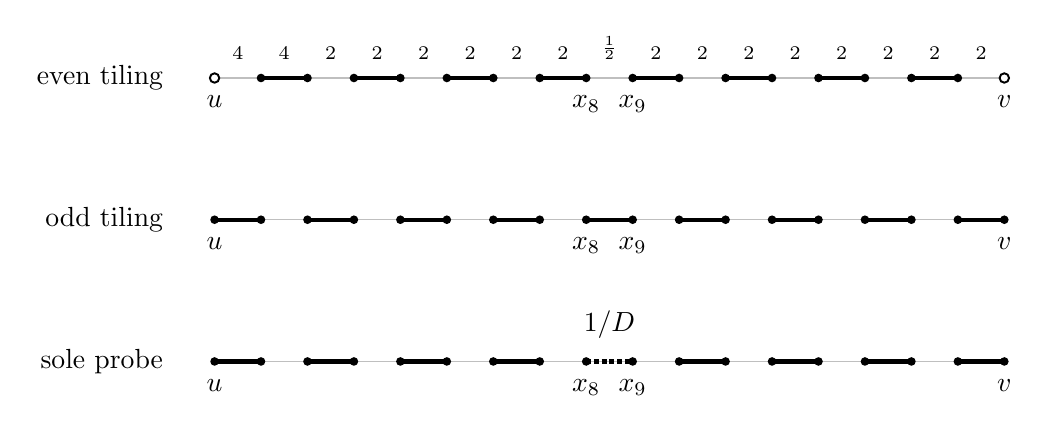
\begin{tikzpicture}[x=.59cm,y=1cm,
  reference/.style={draw=black!25,line width=.45pt},
  selected/.style={draw=black,line width=1.5pt},
  vertex/.style={circle,fill=black,inner sep=1.1pt}]
  \foreach \row/\height in {even/3.6,odd/1.8,probe/0} {
    \foreach \i in {0,...,17} {
      \coordinate (\row\i) at (\i,\height);
    }
    \foreach \j [evaluate=\j as \i using int(\j-1)] in {1,...,17}
      \draw[reference] (\row\i)--(\row\j);
  }
  \foreach \j [evaluate=\j as \i using int(\j-1)] in {2,4,...,16}
    \draw[selected] (even\i)--(even\j);
  \foreach \j [evaluate=\j as \i using int(\j-1)] in {1,3,...,17}
    \draw[selected] (odd\i)--(odd\j);
  \foreach \j [evaluate=\j as \i using int(\j-1)] in {1,3,5,7,11,13,15,17}
    \draw[selected] (probe\i)--(probe\j);
  \draw[draw=black,densely dotted,line width=1.8pt]
    (probe8)--(probe9) node[midway,above=4pt] {$1/D$};
  \foreach \row in {even,odd,probe} {
    \foreach \i in {0,...,17}
      \node[vertex] at (\row\i) {};
    \node[below=3pt] at (\row0) {$u$};
    \node[below=3pt] at (\row8) {$x_8$};
    \node[below=3pt] at (\row9) {$x_9$};
    \node[below=3pt] at (\row17) {$v$};
  }
  \foreach \i in {0,17}
    \draw[fill=white,line width=.7pt] (even\i) circle[radius=1.7pt];
  \foreach \j [evaluate=\j as \i using int(\j-1)] in {1,...,17} {
    \ifnum\j<3
      \node[font=\scriptsize,above=3pt] at ($(even\i)!.5!(even\j)$) {$4$};
    \else\ifnum\j=9
      \node[font=\scriptsize,above=3pt] at ($(even\i)!.5!(even\j)$) {$\tfrac12$};
    \else
      \node[font=\scriptsize,above=3pt] at ($(even\i)!.5!(even\j)$) {$2$};
    \fi\fi
  }
  \node[anchor=east] at (-.9,3.6) {even tiling};
  \node[anchor=east] at (-.9,1.8) {odd tiling};
  \node[anchor=east] at (-.9,0) {sole probe};
\end{tikzpicture}
\caption{One subdivision path with $K=1$, $p=4$ and $4p+1=17$ edges.
The top labels are the real activities: $H_u=4$,
$H_v=B_{uv}=2$, and $\lambda_{uv}=1/2$; the central edge has
effective strength $B'_{x_8x_9}=2$. Solid edges show the selected
real tiling. The even tiling uses neither terminal, and the odd tiling
uses both; the odd-to-even weight ratio is $\lambda_{uv}$.
The last row uses the probe portion of the central colored bag edge
and real portions elsewhere. Here the central label has height $h_l=2$,
so its collapsed activity $1/2+2/D$ consists of real activity $1/2$,
probe activity $1/D$, and remaining virtual activity $1/D$.
The probe forces the real edges on the two outer legs to use both
terminals. Their combined weight equals the even-tiling weight,
so the remaining paths represent a logical matching with $u,v$ deleted.}
\label{fig:subdivision-probe-example}
\end{figure}

Let $Z_{\mathrm{bag}}$ be the colored partition function of the enlarged
graph, and put $I=Z_{\mathrm{bag}}/Z'$. This ratio measures the mass
introduced by the auxiliary edges.

\begin{proposition}[Marked matching laws]\label{prop:marked-laws}
For arbitrary positive logical activities, sample from the bag matching
law and reveal the edge portions as above. The all-real event has
probability $1/I$;
conditional on this event, the decoded logical matching has law
$\pi_\lambda$. For each logical edge $uv$,
\begin{equation}\label{eq:probe}
 \Prb(\text{probe for }uv\text{ is used and all other edges are real})
 =\frac{g_\lambda(uv)}{DI}.
\end{equation}
Conditional on this event, the residual logical matching has the
$\lambda$-weighted perfect-matching law on the vertices other than
$u,v$.
\end{proposition}

\begin{proof}
Revealing portions recovers the weighted law before the real and virtual
activities were collapsed. The all-real matchings have total weight
$Z'=C_0Z_\lambda$, and their normalized law is transported to
$\pi_\lambda$ by \cref{lem:subdivision}.

Now require the probe on the path for $uv$ and real edges everywhere
else. The probe matches $x_{2p}$ to $x_{2p+1}$. The remaining vertices on
its path have unique real tilings: the left one uses $u$, and the right
one uses $v$. Equal adjacent activities in \eqref{eq:path-profile}
show that their combined weight is exactly the even-edge baseline
weight of this path. Other paths incident to $u$ or $v$ must use their
even tilings. The remaining paths retain their even and odd alternatives,
with ratio $\lambda_e$. Consequently these marked
matchings are in bijection with logical matchings missing $u,v$,
and every weight is multiplied by $C_0/D$. Their total mass is
$C_0 Z_\lambda(-uv)/D$. Dividing by $Z_{\mathrm{bag}}=IC_0Z_\lambda$
proves \eqref{eq:probe}; the same constant weight multiplier proves
the conditional-law assertion.
\end{proof}

The identities show what the enlarged graph provides to the counting
algorithm. To use its all-real event with polynomially many samples,
we also need a uniform lower bound on that event's probability.
The next lower-bound estimate requires balance; the construction and
the exact laws above do not.

\begin{proposition}[Bounded inflation]\label{prop:bag-inflation}
If the logical activities are balanced, then
\begin{equation}\label{eq:inflation}
 1\le I\le2.
\end{equation}
\end{proposition}

We prove this bound in the remainder of the section. A collection of
virtual edges leaves a set $U$ of endpoints to be removed from a real
matching. Its added weight must therefore be compared with $g'(U)$.
The next two subsections transfer the logical hole estimate to these
enlarged hole sets.

\subsection{Exact accounting for deleted vertices}

We next describe exactly what deleting internal vertices does to the
logical graph. A path is \emph{broken} if at least one of its internal
vertices is deleted. Let $E_{\mathrm{br}}(U)$ be the set of logical
edges whose paths are broken by a hole set $U$.

Consider the ordered internal holes on a broken path. If a real
completion exists, successive hole indices alternate in parity,
because the intervening internal run must have even order. A first
hole of even index forces the prefix to match the terminal $u$;
we say that this hole \emph{consumes} $u$ and map it to $u$.
A last hole of odd index similarly consumes and maps to $v$.
Remove all consumed holes (zero, one, or two) from the list. The remaining holes
split, in their order, into pairs $(j,k)$ with $j$ odd and $k$ even;
call these \emph{neutral pairs}. There is no ambiguity when the
list has one hole, since it cannot both have even and odd index.

Let $R$ be the set of explicitly deleted terminals together with all
consumed terminals. Feasibility requires these terminals to be
distinct. To each consumed hole $x_j$ assign the factor
\[
 f_j=
 \begin{cases}
 1,&\text{if it maps to its home terminal},\\
 \lambda_e/T_j,&\text{if it maps to the other terminal}.
 \end{cases}
\]
For a neutral pair $(j,k)$ assign
\begin{equation}\label{eq:neutral-factors}
 f_{jk}=
 \begin{cases}
 T_j^{-1},&j,k\le2p,\\
 T_k^{-1},&j,k\ge2p+1,\\
 \lambda_e/(T_jT_k),&j\le2p<k.
 \end{cases}
\end{equation}
Let $F=F(U)$ be the product of all these factors on all broken paths;
an empty product is one. Both $R$ and $F$ depend only on $U$ and
the fixed path profiles, not on a choice of completion.

For a set $E_0$ of logical edges, write
$Z_\lambda(-R;E_0\text{ forbidden})$ for the partition function
after deleting $R$ and forbidding those edges.

\begin{lemma}\label{lem:deletion-accounting}
If an even hole set $U$ has a real completion, then $R$ is even,
$|R|\le|U|$, and
\begin{equation}\label{eq:deletion-identity}
 Z'(-U)
 =C_0 F(U)
 Z_\lambda\bigl(-R;E_{\mathrm{br}}(U)\text{ forbidden}\bigr).
\end{equation}
In particular,
$g'(U)\le F(U)g_\lambda(R)$.
\end{lemma}

\begin{proof}
Fix a broken path. A prefix ending immediately before a first hole
of index $j$ has $j-1$ internal vertices. If $j$ is odd it uses the
even tiling and leaves $u$ unused; if $j$ is even it uses the odd
tiling and consumes $u$. The suffix has the analogous alternatives.
Every run between consecutive holes has a unique tiling, since its
order is even. These parity conditions prove the stated description
of consumed holes and neutral pairs. On each path the number of
consumed holes has the same parity as the number of internal holes.
Adding explicit terminal holes gives $|R|\equiv|U|\pmod2$.
Distinctness and $|R|\le|U|$ follow from feasibility and the fact
that each consumed terminal is charged to a different hole.

For completeness, all factors can be obtained from one prefix
ratio. For even $j$, define
\[
 P(j)=
 \frac{\prod_{i\le j,\ i\text{ odd}}t_i}
      {\prod_{i\le j,\ i\text{ even}}t_i},
 \qquad P(0)=1.
\]
The profile gives
\[
 P(j)=
 \begin{cases}
 1,&j\le2p,\\
 \lambda_e/T_j,&j\ge2p+2.
 \end{cases}
\]
This is the factor for a first even-indexed hole consuming $u$;
reflection gives the factor for a last odd-indexed hole consuming
$v$. For a neutral pair $(j,k)$, its shifted tiling relative to
the even-edge baseline contributes
\[
 \frac{\prod_{i=j+2,j+4,\ldots,k-1}t_i}
      {\prod_{i=j+1,j+3,\ldots,k}t_i}
 =
 \frac{P(k)}{P(j-1)t_j}.
\]
If $j$ is odd on the left, its denominator is $T_j$; if $j$ is odd
on the right, its denominator is $\lambda_e$, also when
$j=2p+1$. Substitution proves \cref{eq:neutral-factors}.
Prefixes and suffixes that do not consume a terminal, and runs
outside these shifted intervals, retain their baseline even edges.
Thus the product $F$ accounts for all changes to the baseline
on broken paths.

Every completion now determines a logical matching on the intact
paths, using exactly the terminals outside $R$. Conversely, take
any logical perfect matching on the vertices outside $R$ that uses
no broken edge. Give its selected intact paths their odd tilings,
give other intact paths their even tilings, and fill all broken
paths by the uniquely forced runs just described. The distinctness
conditions ensure that no terminal is used twice or is both used
and deleted. This reconstructs a real completion and is inverse
to the first map. Its weight is $C_0F$ times the logical weight,
which proves \cref{eq:deletion-identity}. Omitting the forbidden-edge
condition and dividing by \cref{eq:real-partition} gives the inequality.
\end{proof}

\subsection{Charging the pairing capacity}

The deletion identity gives a factor $F(U)$ and a logical hole set $R$.
To transfer the logical bound, we must compare the pairing capacity of
$U$ with that of $R$. The next lemma expresses both capacities through
threshold classes. Throughout the comparison, these classes belong to
the original undeleted graphs, so they are independent of the completion
being counted.

\begin{lemma}[Pairings in a hierarchy]
\label{lem:ultrametric-pairing}
Let $B\ge1$ be a symmetric similarity on a finite vertex set $X$,
satisfying $B_{ij}\ge\min\{B_{ik},B_{kj}\}$. Let $\mathcal C_t$ be
the equivalence classes of $B\ge t$, including singletons.
For every even set $U\subseteq X$,
\begin{equation}
\label{eq:threshold-pairing}
 \log\Phi_B(U)
 =\int_1^\infty\sum_{C\in\mathcal C_t}
       \left\lfloor\frac{|C\cap U|}{2}\right\rfloor\frac{dt}{t}.
\end{equation}
There is one pairing that attains the maximum number of internal pairs
in every threshold class simultaneously.
\end{lemma}

\begin{proof}
For any pairing $Q$,
\[
 \log\prod_{ij\in Q}B_{ij}
 =\int_1^\infty
       |\{ij\in Q:B_{ij}\ge t\}|\,\frac{dt}{t}.
\]
Inside a threshold class $C$, there are at most
$\lfloor |C\cap U|/2\rfloor$ pairs of $Q$, proving the upper bound.

The threshold classes form a laminar family: any two are disjoint or one
contains the other.  Process its finitely many distinct classes from
smaller to larger, starting with the singletons.  In each class, pair
its currently unpaired elements of $U$ arbitrarily until at most one
remains.  When a class $C$ has been processed, exactly
$\lfloor|C\cap U|/2\rfloor$ pairs lie inside it.  Subsequent processing
cannot create another pair inside $C$, because at most one element of
$C\cap U$ remains unpaired.  The final class is $X$, and $|U|$ is even,
so the procedure produces a pairing.  It attains every floor count,
and therefore attains the integral upper bound.
\end{proof}

\begin{lemma}\label{lem:lifted-hole-bound}
If the logical activities are balanced, then for every even set
$U$ of enlarged vertices,
\[
 g'(U)\Phi_{B'}(U)\le2D_0^{|U|/2}.
\]
More precisely, for every $U$ with a real completion, the deterministic
quantities above satisfy
\begin{equation}\label{eq:threshold-charge}
 F(U)\Phi_{B'}(U)\le\Phi_B(R).
\end{equation}
\end{lemma}

\begin{proof}
The assertion is immediate if $U$ has no completion, so suppose
otherwise. For a threshold $t>1$ and any set $A$ of enlarged vertices,
let
\[
 S'_t(A)=\sum_{C}\left\lfloor\frac{|A\cap C|}{2}\right\rfloor,
\]
where $C$ ranges over the threshold classes of $B'$. Define $S_t$ on
logical vertices in the same way using $B$. These definitions make
sense even when $A$ has odd cardinality.
The threshold partitions remain those of the undeleted graphs
throughout this proof; only the sets of holes are changed.

By \cref{lem:subdivision}, an internal vertex $x_j$ is isolated in
the threshold partition precisely when $T_j<t$; otherwise it is
connected to its home terminal. Call it \emph{active} in the latter
case. The threshold relation induced on terminals is exactly the
logical relation. These statements can equivalently be checked using
raw real edges of activity at least $t$, since taking the bottleneck
closure leaves threshold components unchanged.

Remove the neutral pairs one at a time from the current hole set.
For a pair on the same side, its active vertices lie in one class.
Removing it reduces $S'_t$ by at most
\[
 \one_{\{\max(T_j,T_k)\ge t\}}.
\]
Indeed, two active holes are removed from one class, one active hole
reduces a class floor by at most one, and an inactive hole is in
a singleton class and contributes zero. On the left
$\max(T_j,T_k)=T_j$; on the right it is $T_k$. For a cross pair, the
loss is at most
\[
 \one_{\{T_j\ge t\}}+\one_{\{T_k\ge t\}}
 -\one_{\{\lambda_e\ge t\}}.
\]
To see the subtracted term, when $\lambda_e\ge t$ both vertices
are active and are connected by the full path, so their removal
reduces a single class floor by one. Otherwise the bound is the
sum of the separate active-hole bounds. These arguments apply to
the current set after any preceding removals.

Next consider each consumed hole mapping away from home. If it is
active and $\lambda_e<t$, discard it. The floor loss is at most
\[
 \one_{\{T_j\ge t\}}-\one_{\{\lambda_e\ge t\}}.
\]
The expression is nonnegative, since $T_j\ge B_e\ge\lambda_e$.
Every remaining active consumed hole can be mapped to its consumed
terminal within its threshold class: a home mapping always has this
property, and an away mapping retained by the rule has
$\lambda_e\ge t$. Together with explicitly deleted terminals, these
maps are injective, by the distinctness in
\cref{lem:deletion-accounting}. Inactive internal holes lie in
singleton classes and contribute no floor. Hence the floor sum
remaining after the removals and discards is at most $S_t(R)$.

Integrate these bounds against $dt/t$ on $(1,\infty)$. By
\cref{lem:ultrametric-pairing}, the integral of $S'_t(U)$ is
$\log\Phi_{B'}(U)$, and that of $S_t(R)$ is $\log\Phi_B(R)$.
For a same-side neutral pair the integrated charge is exactly
$-\log f_{jk}$. For a cross pair it is
\[
 \log T_j+\log T_k-\log\max\{1,\lambda_e\}
 \le-\log f_{jk}.
\]
For an away-mapped hole it is
\[
 \log T_j-\log\max\{1,\lambda_e\}\le-\log f_j.
\]
Home mappings cost zero. Summing proves
$\log\Phi_{B'}(U)\le\log\Phi_B(R)-\log F$,
which is \cref{eq:threshold-charge}. Finally,
\cref{lem:deletion-accounting,thm:logical-hole-bound} give
\[
 g'(U)\Phi_{B'}(U)
 \le g_\lambda(R)\Phi_B(R)
 \le2D_0^{|R|/2}
 \le2D_0^{|U|/2}.
\]
\end{proof}

\begin{proof}[Proof of \cref{prop:bag-inflation}]
Expand the partition function before collapsing real and virtual
portions. A nonempty partial matching $Q$ of $a$ colored virtual
edges, with endpoint set $U$, contributes relative to $Z'$ the mass
\[
 g'(U)\prod_{xy,l\in Q}\frac{h_l}{D}.
\]
Vertices sharing $l$ lie in the same threshold component at $h_l$,
so $h_l\le B'_{xy}$. Their pairing therefore gives
\[
 g'(U)\prod_{xy,l\in Q}\frac{h_l}{D}
 \le D^{-a}g'(U)\Phi_{B'}(U)
 \le2(D_0/D)^a
\]
by \cref{lem:lifted-hole-bound}. A vertex pair has at most two
common labels, so there are fewer than $N^2$ colored virtual edges
and at most $N^{2a}$ choices for $Q$. The empty $Q$ contributes one.
Consequently,
\[
 1\le I\le1+2\sum_{a\ge1}(N^2D_0/D)^a
 =1+\frac2{99}<2.
\]

\end{proof}

\section{A quadrangulation adapted to the labels}
\label{sec:cells}

We now turn to the sampling branch of the proof. Its input is a
tree-bag graph as in \cref{def:tree-bags}; no balance assumption is
needed. To compare two alternating matchings on a cycle, we shall
subdivide its polygon into four-corner cells. A cell side may stand
for a long arc of the original cycle. We first describe the matching
patterns on such an arc and the endpoint repairs the cells must
permit, then construct a quadrangulation with those properties.

Let $\mathcal C$ be a simple even cycle of length $m\ge4$ in the colored
bag graph.  Each edge retains its color, which is a node of the label
tree.  For a vertex $v$ of $\mathcal C$, define
\[
 S_v=\{\text{labels of the two edges of $\mathcal C$ incident to $v$}\}.
\]
Thus $S_v$ is a singleton or consists of two adjacent tree nodes.
These sets refer to the \emph{original full cycle} throughout the
construction; adding a diagonal never changes them.  In particular,
the cyclic sequence of edge labels is a walk on the tree, with repetitions
allowed.

An \emph{arc} is one of the two paths in $\mathcal C$ between distinct
vertices, specified together with its endpoints. Its length is its
number of edges. We use only odd arcs. An arc is \emph{admissible} if
its endpoints $u,v$ satisfy $S_u\cap S_v\ne\varnothing$. The clique
property then supplies an edge joining them with any chosen label in
this intersection.

For an admissible odd arc $J=(v_0,\ldots,v_s)$, choose such a colored
endpoint chord $e_J$ and put
\[
 T_J=\{v_0v_1,v_2v_3,\ldots,v_{s-1}v_s\},\qquad
 N_J=\{v_1v_2,v_3v_4,\ldots,v_{s-2}v_{s-1}\},
 \qquad C_J=N_J\cup\{e_J\}.
\]
All path edges retain their cycle colors. The \emph{through pattern}
$T_J$ and the \emph{closed pattern} $C_J$ both perfectly match the
vertices of $J$; the \emph{interior pattern} $N_J$ leaves only its
two endpoints unmatched. The symbol $C_J$ denotes a matching, not the
original cycle. Call $J$ \emph{short} if $s=1$ and \emph{long} otherwise.
On a short arc choose its actual cycle edge as $e_J$, so $T_J=C_J$.
When a diagonal later represents two complementary arcs, we use the
same colored chord in both patterns. \Cref{fig:odd-arc-patterns} shows
these patterns on a long arc.

\begin{figure}[ht]
\centering
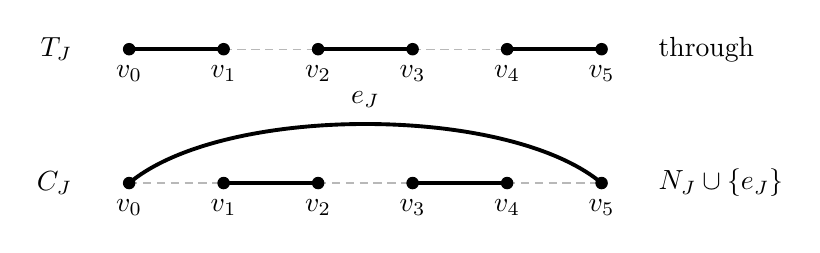
\begin{tikzpicture}[x=1.2cm,y=1cm,
  reference/.style={draw=black!28,densely dashed,line width=.5pt},
  selected/.style={draw=black,line width=1.4pt},
  vertex/.style={circle,fill=black,inner sep=1.6pt}]
  \foreach \i in {0,...,5} {
    \coordinate (t\i) at (\i,1.7);
    \coordinate (c\i) at (\i,0);
  }
  \foreach \i [evaluate=\i as \j using int(\i+1)] in {0,...,4} {
    \draw[reference] (t\i)--(t\j);
    \draw[reference] (c\i)--(c\j);
  }
  \foreach \i [evaluate=\i as \j using int(\i+1)] in {0,2,4}
    \draw[selected] (t\i)--(t\j);
  \foreach \i [evaluate=\i as \j using int(\i+1)] in {1,3}
    \draw[selected] (c\i)--(c\j);
  \draw[selected] (c0) .. controls +(1,1) and +(-1,1) .. (c5)
    node[pos=.5,above=2pt] {$e_J$};
  \foreach \i in {0,...,5} {
    \node[vertex,label=below:{$v_{\i}$}] at (t\i) {};
    \node[vertex,label=below:{$v_{\i}$}] at (c\i) {};
  }
  \node[anchor=east] at (-.5,1.7) {$T_J$};
  \node[anchor=east] at (-.5,0) {$C_J$};
  \node[anchor=west] at (5.5,1.7) {through};
  \node[anchor=west] at (5.5,0) {$N_J\cup\{e_J\}$};
\end{tikzpicture}
\caption{The two patterns on a long odd arc, illustrated for
$J=(v_0,\ldots,v_5)$. Solid edges form the indicated matching;
faint dashed edges only locate the underlying path. Both $T_J$ and
$C_J$ perfectly match the same vertices. The latter uses the interior
pattern $N_J$ and the endpoint chord $e_J$; their union
$T_J\cup C_J$ is the alternating cycle consisting of $J$ and its chord.
Replacing $T_J$ by $C_J$ can change interior edges; this replacement
need not be a single chain update.}
\label{fig:odd-arc-patterns}
\end{figure}

Besides closing an arc with a chord, we shall sometimes need to free
its endpoints while starting from its through pattern. Removing the
first and last edges of a long arc from $T_J$ uncovers its endpoints
and its two \emph{leaves} $v_1,v_{s-1}$. Call $J$ \emph{good} if it is
short or if
\[
 S_{v_1}\cap S_{v_{s-1}}\ne\varnothing.
\]
For a good long arc, choose an edge between its leaves with a label in
this intersection, called a \emph{leaf repair}. After the two boundary
edges are removed, inserting this repair matches all internal vertices
and leaves both endpoints free. For a short arc, deleting its sole
edge does the same. This is the matching operation encoded by the
good-arc condition. The \emph{boundary edges of an arc} mean only its
first and last edges, which coincide for a short arc.

Realize the vertices of $\mathcal C$ in their cyclic order as a convex
polygon.  A quadrangulation is a subdivision of this polygon into
quadrilaterals by noncrossing diagonals.  A side of a cell represents the
arc of the original cycle from one corner to the next corner, containing
no other corner of that cell.  Consequently the four sides of each cell
represent four consecutive arcs partitioning the entire cycle.  An
interior diagonal has two occurrences as a cell side, and their arcs
are complementary in the original cycle.

\begin{lemma}[Label-adapted quadrangulation]
\label{lem:quadrangulation}
The polygon of $\mathcal C$ has a quadrangulation such that every cell
side represents an admissible odd arc and the following hold in every
cell:
\begin{enumerate}[label=\textup{(\roman*)}]
 \item some opposite pair of sides consists of good arcs;
 \item if both arcs in an opposite pair are long, both arcs in the
 other opposite pair are good.
\end{enumerate}
There are $(m-2)/2$ cells and $(m-4)/2$ interior diagonals.  One can
construct the quadrangulation in time polynomial in $m$ and the encoding
length of the label tree.

Each diagonal may be assigned any common label from the fixed sets at
its endpoints, used consistently in its two occurrences.  For a short
side, use the color of its actual cycle edge.  These choices need not
coincide with the auxiliary labels used in the construction.
\end{lemma}

\begin{proof}
We give a recursive splitting rule.  A subproblem is an admissible odd
arc $J=(v_0,\ldots,v_s)$; its \emph{exterior} is its complementary arc
in the full cycle.  Choose a label $P\in S_{v_0}\cap S_{v_s}$, and
write $a_i$ for the label of $v_iv_{i+1}$, $0\le i<s$.
Adjacent terms of this sequence are equal or adjacent in the tree.
If $s=1$, no cell is needed.  For $s\ge3$, we find indices
\begin{equation}
\label{eq:cell-split-indices}
 0<p_1<p_2<s,\qquad p_1\text{ odd},\quad p_2\text{ even},
\end{equation}
such that the three subarcs with successive endpoint pairs
\[
 (v_0,v_{p_1}),\qquad (v_{p_1},v_{p_2}),\qquad
 (v_{p_2},v_s)
\]
are admissible.  They and the exterior arc form the four sides of the
new cell.  We call these the first, middle, third, and exterior sides,
respectively.

We repeatedly use the following elementary fact about a tree.
If a contiguous part of the label walk avoids $P$ and its first and
last labels are adjacent to $P$, these two labels coincide: the walk
lies in a single component of the tree with $P$ removed, and that
component has just one node adjacent to $P$.

\paragraph{The exterior is good.}
It suffices to make either the middle side short or both the first and
third sides short.  Either alternative immediately implies
\textup{(i)} and \textup{(ii)}, because the exterior is good.

First ensure that some $a_i$ equals $P$.  If none does, $a_0$ and
$a_{s-1}$ are adjacent to $P$, because the endpoint sets contain $P$.
The elementary tree fact gives $a_0=a_{s-1}=Q$ for a neighbor $Q$ of
$P$.  Replace $P$ by $Q$, which also lies in both endpoint sets.
We now distinguish the exhaustive possibilities below.
\begin{enumerate}[label=\textup{(\alph*)}]
 \item Suppose $a_i=P$ for an odd $i$.
 Set $p_1=i$ and $p_2=i+1$.  The middle side is short.  The first
 side's two endpoints contain $P$, as do the third side's two
 endpoints, so all three sides are admissible.

 \item Otherwise all occurrences of $P$ have even indices.
 If their first index is $i>0$, set $p_1=i-1$ and $p_2=i$.
 The prefix $a_0,\ldots,a_{i-1}$ avoids $P$, and its first and last
 labels are adjacent to $P$.  They therefore equal the same neighbor
 $Q$.  The first side's endpoints both contain $Q$, and the third
 side's endpoints both contain $P$.  The middle side is short.

 \item Suppose the first occurrence is at $0$, but the last occurrence
 is at $j<s-1$.  Set $p_1=j+1$ and $p_2=j+2$.
 The suffix $a_{j+1},\ldots,a_{s-1}$ avoids $P$ and has its two end
 labels adjacent to $P$, so they equal one neighbor $Q$.
 The first side's endpoints contain $P$, the third side's endpoints
 contain $Q$, and the middle side is short.

 \item In the remaining case $a_0=a_{s-1}=P$.
 Set $p_1=1$ and $p_2=s-1$.  Both outer sides are short, and the
 middle side's endpoints both contain $P$.
\end{enumerate}
All indices satisfy \eqref{eq:cell-split-indices}.  For example, in
\textup{(b)} the even index $i$ is at least $2$, and in \textup{(c)}
the even index $j$ is at most $s-3$.

\paragraph{The exterior is not good.}
The exterior is then long.  At least one of its leaves lacks $P$ in
its fixed label set, since otherwise its two leaves would share $P$.
Reverse the indexing of $J$ if necessary so that this leaf is the
exterior neighbor of $v_0$.  The exterior edge at $v_0$ cannot have
label $P$.  Since $P\in S_{v_0}$, the first edge of $J$ must have
label $a_0=P$.

If $a_{s-1}=P$ as well, choose $p_1=1,p_2=s-1$.  Both outer sides
are short, and the middle side is admissible.  Otherwise let $t-1$
be the last index with $a_{t-1}=P$.  Thus $1\le t\le s-1$.
The suffix $a_t,\ldots,a_{s-1}$ avoids $P$.  Its first label is
adjacent to $P$, and its last label is adjacent to $P$ because
$P\in S_{v_s}$.  Hence
\[
 a_t=a_{s-1}=Q
\]
for the same neighbor $Q$ of $P$.
\begin{itemize}
 \item If $t$ is even, set $p_1=1,p_2=t$.
 The first side is short.  The middle side's endpoints both contain
 $P$, and the third side's endpoints both contain $Q$.
 The third side is good: if long, both its boundary edges have
 label $Q$, so both its leaves contain $Q$.

 \item If $t$ is odd, set $p_1=t,p_2=s-1$.
 The third side is short.  The first side's endpoints both contain
 $P$, and the middle side's endpoints both contain $Q$.
 The first side is good because, if long, both its boundary edges
 have label $P$.
\end{itemize}
The required strict inequalities follow from $t\ge2$ in the even
case and $t\le s-2$ in the odd case.  In either case the first and
third sides are good and at least one is short.  This proves
\textup{(i)}.  The only opposite pair that can contain two long sides
is the middle--exterior pair, and its other pair is good, proving
\textup{(ii)}.

\paragraph{Recursion and consistent diagonals.}
Start with any arc of length $m-1$, whose exterior is the remaining
single cycle edge.  Its endpoints share that edge's label.
Apply the splitting rule and recurse on each of the three subarcs
whose length exceeds one, always using the original sets $S_v$ and
the complement in the original cycle as exterior.  The three
subpolygons have disjoint interiors, so all diagonals are noncrossing.
Each recursive child has odd length and admissible endpoints by the
construction.  The splitting label $P$ is only an auxiliary witness
to admissibility; it does not constrain the color of the closing
diagonal.  Thus each diagonal can be colored once and the same color
used on both sides.

For an odd arc of length $s$, the resulting number of cells is
$(s-1)/2$: this is zero for $s=1$, and a split into odd lengths
$s_1+s_2+s_3=s$ gives
\[
 1+\sum_{i=1}^{3}\frac{s_i-1}{2}=\frac{s-1}{2}.
\]
The root therefore gives $(m-2)/2$ cells.  Each nonroot recursive
subproblem that creates a cell has one closing diagonal, giving one
fewer interior diagonals than cells. A direct implementation scans
at most $m$ labels in each of the $(m-2)/2$ nontrivial subproblems;
the recursion also has $m-1$ short leaf arcs. Fixing total orders for
any choices makes the construction deterministic, with $O(m^2)$
label comparisons and polynomial bit cost.
\end{proof}

For each cell, choose its colored side chords as in
\cref{lem:quadrangulation}; for each good long side, choose one leaf
repair.  These are precisely the additional edges needed for the
local matching constructions in the next section.

\begin{lemma}[Comparability within a cell]
\label{lem:cell-comparability}
Consider the four colored side chords of a cell, the first and last
cycle edges of each of its four arcs, and one leaf repair for each
good long arc.  The labels of any two edges in this collection have
tree distance at most $6$.  Consequently their activities lie within
a factor
\[
 A_0=1000D
\]
of one another.  The same conclusion holds after clamping every edge
activity to any common interval $[a,b]\subset(0,\infty)$.
\end{lemma}

\begin{proof}
Two consecutive side chords have labels in the same fixed set $S_v$
at their common cell corner, so their labels are equal or adjacent.
Any two of the four side-chord labels therefore have distance at
most $2$.  A boundary edge of an arc and its side chord have labels
in the same $S_v$ at the relevant endpoint, giving distance at most
$1$.  A leaf repair and the boundary edge at either of its leaves
have labels in that leaf's fixed set, again giving distance at most
$1$.  Thus each edge in the stated collection is at distance at
most $2$ from its side chord, and the diameter is at most
$2+2+2=6$.

Adjacent labels have heights differing by a factor $2$.  If edges
$e,f$ have labels $\ell,\ell'$ with distance at most $6$, the
assumed activity bounds imply
\[
 \frac{W_e}{W_f}
 \le \frac{3h_\ell}{h_{\ell'}/D}
 \le 3D\,2^6=192D\le A_0.
\]
The same bound holds with $e,f$ exchanged.  Finally the common clamp
$\psi(x)=\max\{a,\min\{b,x\}\}$ satisfies
\[
 1\le\frac{\psi(x)}{\psi(y)}\le\frac{x}{y}
 \qquad (x\ge y>0).
\]
For example this follows by observing that
$\log\psi(e^u)$ is the clamp of $u$ to
$[\log a,\log b]$, a nondecreasing $1$-Lipschitz function.
Clamping therefore preserves the factor bound.
\end{proof}
\section{A two-coordinate energy inequality}
\label{sec:energy}

This section proves the sampling argument's main inequality. The four
side chords of each cell give a two-edge switch whose changed edges
have comparable activities. Long arc conversions are used in an exact
signed identity and need not be individual chain moves. We control the
resulting context errors by swapping an alternating cycle with an
independent matching. Encodings by two matchings change only a bounded
number of edges in their multiset union, and their preimage counts give
polynomial load bounds.
The variance-to-energy comparison is related to the flow method
of~\cite{Sinclair1992}, but we do not invoke a path-congestion theorem:
the signed identity and its context-error estimates are established
for the present pair kernel.

Fix a tree-bag graph on $N\ge2$ vertices, with at least one perfect
matching, and let $w$ be either its reference activities or any common
clamp of them.  Write $\pi(M)=\wt_w(M)/Z_w$ and $\calM$ for its colored
perfect matchings.  Throughout this section put
\begin{equation}
\label{eq:energy-constants}
 A_0=1000D,\qquad \calT=(10N)^{30},\qquad
 L=(10^4ND)^{100}.
\end{equation}

\subsection{The pair kernel}

On $(A,B)\in\calM^2$, choose each of the following proposal types with
probability $1/3$.
\begin{enumerate}[label=\textup{(\arabic*)}]
 \item \emph{Two-edge switch.}  Choose an unordered pair of distinct
 edges of $A$ uniformly, and choose either alternative pairing of
 their four endpoints with probability $1/2$.  For each proposed
 edge, choose index $1$ or $2$ with probability $1/2$ from the ordered
 list of common labels of its endpoints.  If an index is absent,
 stay put.  If $A$ has fewer than two edges, stay put.

 \item \emph{Color change.}  Choose an edge of $A$ uniformly and
 choose index $1$ or $2$ from the common-label list with probability
 $1/2$.  An absent index gives a holding move.

 \item \emph{Cycle swap.}  Choose uniformly one discrepancy cycle of
 $A,B$ and interchange its two layers.  If there is no discrepancy
 cycle, stay put.
\end{enumerate}
Accept each proposal by the Metropolis rule for $\pi\otimes\pi$.
Denote the resulting kernel by $P$ and its energy by $\calE$.
The proposal is symmetric.  For the first two types, the reverse
choice has the same edge, pairing, and color-index probabilities;
the possible holding choices do not change this fact.  For the third
type, the discrepancy cycles and their number are unchanged by the
swap.  In particular, a cycle swap always has acceptance probability
one, since its product weight is unchanged.

\begin{theorem}[Pair energy inequality]
\label{thm:pair-energy}
For every two real functions $f_1,f_2$ on $\calM$,
\begin{equation}
\label{eq:pair-energy}
 \Var_\pi f_1\le L\,
 \calE\bigl((A,B)\mapsto f_1(A)+f_2(B)\bigr).
\end{equation}
The same constant works for every common-interval clamp of the
reference activities.
\end{theorem}

In the proof write $F(A,B)=f_1(A)+f_2(B)$ and $E=\calE(F)$.
A two-edge switch is called \emph{safe} if its four removed or
inserted colored edges have activities within a factor $A_0$ of one
another.  Let $\mathcal S(A)$ be its possible safe destinations, and
let $\mathcal K(A)$ be its possible destinations by changing one
edge color.  Consecutive labels have comparable heights, so every
color change has activity ratio in $[A_0^{-1},A_0]$.

\begin{lemma}[Elementary energy bounds]
\label{lem:elementary-pair-energy}
With the notation above,
\begin{align}
 \sum_A\pi(A)\sum_{A'\in\mathcal S(A)}
       (f_1(A)-f_1(A'))^2
 &\le60N^2A_0^2 E,
 \label{eq:safe-switch-energy}\\
 \sum_A\pi(A)\sum_{A'\in\mathcal K(A)}
       (f_1(A)-f_1(A'))^2
 &\le12NA_0 E,
 \label{eq:color-energy}\\
 \sum_{A,B}\pi(A)\pi(B)\sum_{C\in\mathcal C(A,B)}
       \bigl(F(A,B)-F((A,B)^C)\bigr)^2
 &\le6NE.
 \label{eq:cycle-energy}
\end{align}
Here $\mathcal C(A,B)$ denotes the discrepancy cycles, and $(A,B)^C$
is the pair after swapping $C$.
\end{lemma}

\begin{proof}
Every specified legal two-edge switch has proposal probability
at least $1/(30N^2)$; its Metropolis acceptance is at least
$A_0^{-2}$ when safe.  Every specified color change has proposal
probability at least $1/(6N)$ and acceptance at least $A_0^{-1}$.
These moves change only the $f_1$ summand of $F$, so summing the
second-coordinate law and using the factor $1/2$ in the energy proves
the first two bounds.  There are at most $N$ discrepancy cycles.
Each specified swap therefore has proposal probability at least
$1/(3N)$ and is accepted; this proves the third bound.
\end{proof}

\subsection{An exact identity on a cycle}

Fix a pair of demand matchings $(I_1,I_2)$ and a simple discrepancy
cycle $C$ of length at least four.  All orientations and choices below
are deterministic, using the orders fixed in \cref{sec:preliminaries}.
Let $R$ be the edges of $I_1$ outside $C$, and let $O_0=I_1$ and
$O_1$ be the matching obtained by toggling $C$ in $I_1$.  Thus both
orientations use $R$ outside $C$.  Put
\[
 D_C=f_1(O_0)-f_1(O_1).
\]
Apply \cref{lem:quadrangulation} and fix the colors of its diagonals
consistently.  A cell's four sides always mean the four odd arcs of
the \emph{original whole cycle}, not paths formed from earlier
diagonals.

Use the through, interior, and closed patterns $T_J,N_J,C_J$ from
\cref{sec:cells}, with the chosen chord colors. A side $J$ is
\emph{through} in $O_\varepsilon$ if $T_J\subseteq O_\varepsilon$.
Exactly one orientation $O_\varepsilon$ contains $T_J$; define
\begin{equation}
\label{eq:canonical-gain}
 H_J=(O_\varepsilon\setminus T_J)\cup C_J,
 \qquad g_J=f_1(O_\varepsilon)-f_1(H_J).
\end{equation}
For a short side, the chord is its actual cycle edge, so $g_J=0$.

The reason for using the original cycle on every cell side is already
visible on a six-cycle $C=(v_0,\ldots,v_5,v_0)$. Take
\[
 O_0=R\cup\{v_0v_1,v_2v_3,v_4v_5\},\qquad
 O_1=R\cup\{v_1v_2,v_3v_4,v_5v_0\},
\]
and suppose the diagonal $e=v_0v_3$ is admissible. In the two cells
it represents the complementary arcs
$J=(v_3,v_4,v_5,v_0)$ and $\bar J=(v_0,v_1,v_2,v_3)$, respectively.
Both conversions yield the same matching
\[
 H_J=H_{\bar J}=H=R\cup\{v_1v_2,e,v_4v_5\}.
\]
Thus $g_{\bar J}-g_J=f_1(O_0)-f_1(O_1)=D_C$; the shared diagonal
contributes one whole-cycle difference, not zero.
\Cref{fig:complementary-arcs} displays this common converted matching.
This example isolates the complementary-gain identity. Its cells have
only one long side each, so the context errors introduced below vanish;
cells with two opposite long sides require a further estimate.

\begin{figure}[ht]
\centering
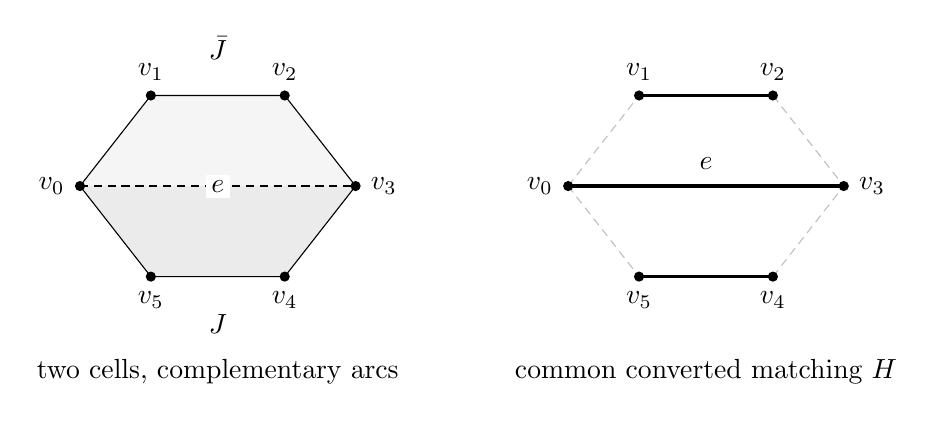
\begin{tikzpicture}[x=1cm,y=1cm,
  vertex/.style={circle,fill=black,inner sep=1.3pt},
  selected/.style={draw=black,line width=1.3pt}]
  \foreach \prefix/\shift in {a/0,b/6.2} {
    \coordinate (\prefix0) at (\shift,0);
    \coordinate (\prefix1) at (\shift+.9,1.15);
    \coordinate (\prefix2) at (\shift+2.6,1.15);
    \coordinate (\prefix3) at (\shift+3.5,0);
    \coordinate (\prefix4) at (\shift+2.6,-1.15);
    \coordinate (\prefix5) at (\shift+.9,-1.15);
  }
  \fill[black!4] (a0)--(a1)--(a2)--(a3)--cycle;
  \fill[black!8] (a0)--(a3)--(a4)--(a5)--cycle;
  \draw (a0)--(a1)--(a2)--(a3)--(a4)--(a5)--cycle;
  \draw[densely dashed,line width=.8pt] (a0)--(a3)
    node[midway,fill=white,inner sep=2pt] {$e$};
  \node at (1.75,1.75) {$\bar J$};
  \node at (1.75,-1.75) {$J$};
  \draw[black!25,densely dashed]
    (b0)--(b1)--(b2)--(b3)--(b4)--(b5)--cycle;
  \draw[selected] (b1)--(b2);
  \draw[selected] (b0)--(b3) node[midway,above=2pt] {$e$};
  \draw[selected] (b4)--(b5);
  \foreach \prefix in {a,b} {
    \node[vertex,label=left:{$v_0$}] at (\prefix0) {};
    \node[vertex,label=above:{$v_1$}] at (\prefix1) {};
    \node[vertex,label=above:{$v_2$}] at (\prefix2) {};
    \node[vertex,label=right:{$v_3$}] at (\prefix3) {};
    \node[vertex,label=below:{$v_4$}] at (\prefix4) {};
    \node[vertex,label=below:{$v_5$}] at (\prefix5) {};
  }
  \node at (1.75,-2.35) {two cells, complementary arcs};
  \node at (7.95,-2.35) {common converted matching $H$};
\end{tikzpicture}
\caption{An admissible diagonal $e=v_0v_3$ cuts a six-cycle into two
cells. In the upper cell its side follows the lower boundary arc $J$;
in the lower cell its side follows the upper boundary arc $\bar J$.
The two occurrences use the same colored edge $e$. Converting the
through pattern on either arc gives the restriction of $H$ shown on
the right (the common outside matching $R$ is omitted),
so their signed gains sum to $D_C$. The drawing concerns the signed
identity, not a sequence of chain transitions.}
\label{fig:complementary-arcs}
\end{figure}


In a cell, let $P$ be its opposite pair of sides through in $O_0$,
and $Q$ its opposite pair through in $O_1$.  Let $A_P$ use $N_J$ on
every side and the chords of the two sides of $P$, together with $R$.
Define $A_Q$ analogously and put
\[
 \Delta=f_1(A_P)-f_1(A_Q).
\]
These are legal perfect matchings: the interior vertices are matched
by the $N_J$'s, and the two chosen chords match the four corners.
Their difference is a safe two-edge switch by
\cref{lem:cell-comparability}.

Order each opposite pair as $(Y,X)$.  For the orientation in which
both are through, first convert $Y$ and then $X$.
Write $A^{(0)}=O_\varepsilon$ and $A^{(1)}=H_Y$ for the two
pre-conversion contexts of $X$.  For a matching $R'$ on the vertices
outside $X$, define
\begin{equation}
\label{eq:arc-derivative}
 \partial_X f(R')=f(T_X\cup R')-f(C_X\cup R').
\end{equation}
The context error of the ordered opposite pair is
\begin{equation}
\label{eq:context-error}
 E_{Y,X}
 =\partial_X f_1(A^{(1)}\setminus T_X)
  -\partial_X f_1(A^{(0)}\setminus T_X).
\end{equation}
It is zero if either side is short.  Denote these errors by $E_P,E_Q$
for the two ordered pairs of the cell.

\begin{lemma}[Cell identity and cancellation]
\label{lem:cell-identity}
The quantities just defined satisfy
\begin{equation}
\label{eq:single-cell-identity}
 D_C=\Delta+\sum_{J\in P}g_J-\sum_{J\in Q}g_J+E_P-E_Q
\end{equation}
for each cell.  Consequently,
\begin{equation}
\label{eq:global-cell-identity}
 D_C=\sum_{\text{cells of }C}(\Delta+E_P-E_Q).
\end{equation}
\end{lemma}

\begin{proof}
The first conversion in an opposite pair has its canonical gain.
The second has its canonical gain plus the error in
\eqref{eq:context-error}.  Thus
\[
 f_1(O_0)-f_1(A_P)=\sum_{J\in P}g_J+E_P,
 \qquad
 f_1(O_1)-f_1(A_Q)=\sum_{J\in Q}g_J+E_Q.
\]
Subtracting proves \eqref{eq:single-cell-identity}.

Consider an interior diagonal with complementary arcs $J,\bar J$.
They are through in opposite whole-cycle orientations, and their
converted matchings coincide:
\[
 H_J=H_{\bar J}=R\cup N_J\cup N_{\bar J}\cup\{e_J\}.
\]
Therefore the two signed canonical gains contributed by this
diagonal sum to $f_1(O_0)-f_1(O_1)=D_C$.  The signs here are precisely
those in \eqref{eq:single-cell-identity}: the arc through in $O_0$
has positive sign and the other negative sign.  Boundary sides have
zero gain.  Summing \eqref{eq:single-cell-identity} over the cells
therefore gives one copy of $D_C$ per cell on the left and one per
interior diagonal on the right, in addition to the displayed local
terms.  The number of cells is one more than the number of diagonals,
which proves \eqref{eq:global-cell-identity}.
\end{proof}

\subsection{Encoding the demands}

A \emph{switch demand} specifies $(I_1,I_2)$, a simple discrepancy
cycle $C$, and one cell of its fixed quadrangulation.  Its value is
$\Delta$ above.  An \emph{error demand} specifies these data and one
opposite pair with two long sides, in its fixed order $(Y,X)$.
Its value is $E_{Y,X}$.  The weight of either demand is
$\rho(d)=\pi(I_1)\pi(I_2)$.  Repeated demands from different cells or
different cycles are included separately in all sums.

\begin{lemma}[Encodings with a bounded number of preimages]
\label{lem:encoding}
Every switch demand has an encoding $(A_P,B)$ by two perfect
matchings, and every error demand has encodings
$(A^{(j)},B^{(j)})$ for $j=0,1$, with the following properties.
\begin{enumerate}[label=\textup{(\roman*)}]
 \item For each encoding $(A,B)$,
 $\rho(d)\le A_0^4\pi(A)\pi(B)$.
 \item For each encoding type and each fixed output pair, there are
 at most $\calT$ demand preimages.  This bound includes the choices
 of cycle, cell, opposite pair, and context.
 \item For an error demand, both guide matchings satisfy
 $C_X\subseteq B^{(j)}$.
\end{enumerate}
\end{lemma}

\begin{proof}
We first describe a repair operation.  Start with the union of the
four through patterns $T_J$ in a cell.  Each corner is covered twice,
once by each incident side.  Select a good opposite pair of sides.
For each selected short side delete its sole edge.  For each selected
long side delete its first and last edges, and insert its chosen leaf
repair.  Each corner loses exactly one incident edge.  On a long
selected side the only newly uncovered internal vertices are its
two leaves, which the repair matches.  Thus the resulting edges form
a perfect matching of all cycle vertices.  This verifies legality
also for a side of length three: its two leaves are distinct and
its repair is an ordinary colored edge between them.

\paragraph{Switch demands.}
Use $A_P$ as the first output.  In the second output retain the edges
of $I_2$ outside $C$, start with all four through patterns, and apply
the preceding repair operation to a good opposite pair, which exists
by \cref{lem:quadrangulation}(i).  Call the result $B$.
Before these modifications, the original multiset union contains
exactly one $T_J$ and one $N_J$ on each side.  The output union adds
the two $P$-chords and the leaf repairs and drops the selected boundary
edges.  If $r\in\{0,1,2\}$ selected sides are long, the numbers added
and dropped are both $2+r\le4$.

\paragraph{Error demands, context zero.}
The first output is $A^{(0)}=O_\varepsilon$, the canonical orientation
in which $X,Y$ are through.  Start the second output with the
complementary cycle orientation and the edges of $I_2$ outside $C$.
It has the $N$ patterns on $X,Y$.  Insert their two chords.  The
other opposite pair is good by \cref{lem:quadrangulation}(ii),
because $X,Y$ are both long.  On that other pair delete boundary
edges and insert leaf repairs as above.  The result is a perfect
matching $B^{(0)}$, containing both $C_X$ and $C_Y$.  Again, the
multiset union differs from the original by equally many added
and dropped edges, at most four of each.

\paragraph{Error demands, context one.}
Interchange the patterns $T_Y$ and $C_Y$ between
$A^{(0)},B^{(0)}$.  Each pattern perfectly matches the entire vertex
set of $Y$, so the interchange is legal and gives
$A^{(1)}=H_Y$ and a guide $B^{(1)}$.  The vertex sets of the opposite
arcs $X,Y$ are disjoint; hence $B^{(1)}$ still contains $C_X$.
This interchange does not change the multiset union or product weight.

In every case all added and dropped edges are among the chords,
boundary edges, and good-side leaf repairs of this one cell.
They have pairwise activity ratio at most $A_0$ by
\cref{lem:cell-comparability}.  Since the two lists have equal
length at most four, the input product weight is at most $A_0^4$
times the output product weight.  Division by $Z_w^2$ proves (i).

For completeness we give an inverse, including the information it
needs.  Attach a tag consisting of the four cell corners in cyclic
order, lists of the added and dropped colored edges padded to length
four each, one orientation bit, and fixed flags for the encoding type
(switch, error context zero, or error context one), opposite pair, and
order.  An edge in these lists is an occurrence in
the multiset union; coincident colored edges retain their multiplicities.
Given the output pair and tag, remove the added occurrences and
reinsert the dropped occurrences in its multiset union.  This recovers
the original colored union $I_1\uplus I_2$.  Its component containing
the first tagged corner is the active simple cycle $C$.  The
orientation bit specifies which of the two alternating classes at
that corner belongs to $I_1$, so alternation determines both original
layers on all of $C$.  Outside $C$, the output layers were unchanged;
they recover $I_1,I_2$ there directly.  The fixed quadrangulation can
now be reconstructed.  Its tagged corners identify the cell, and
the flags identify the term and, if appropriate, its ordered pair.
Thus this is an inverse on every tag produced by the construction.

There are at most $2N^2$ possible colored edges.  Allowing a padding
symbol, the tags have at most
\[
 128N^4(1+2N^2)^8
 \le128\cdot3^8N^{20}< (10N)^{30}=\calT
\]
possibilities for $N\ge2$.  Here the factor $128$ more than covers
the orientation bit and the fixed flags; the lists themselves may
be stored in the fixed colored-edge order.  This proves (ii), and
the constructions already proved (iii).
\end{proof}

The encodings provide two kinds of control. Their bounded preimage
count converts a sum over demands to a sum over pairs of matchings.
For context errors, the guide also contains a prescribed closed arc;
this additional condition must survive that summation. We use the
bounded preimage count for switches below, then retain the closed-arc
condition when treating context errors in the next subsection.

We apply this lemma first to switches.  For a fixed encoded pair
$(A,B)$ there are at most $\calT$ demands, and each has its associated
destination $A_Q$ in $\mathcal S(A)$.  Therefore
\begin{align}
 \sum_{d\text{ switch}}\rho(d)\Delta_d^2
 &\le A_0^4\calT\sum_{A,B}\pi(A)\pi(B)
       \sum_{A'\in\mathcal S(A)}(f_1(A)-f_1(A'))^2 \notag\\
 &\le60N^2A_0^6\calT E.
 \label{eq:switch-demand-load}
\end{align}

\subsection{Controlling context errors by cycle swaps}

Here an identity $X$ means a directed, colored, simple odd path of
length at least three together with a specified colored edge joining
its endpoints.  It determines $T_X,C_X$ and \eqref{eq:arc-derivative}.
We may sum over all such identities: this is a finite proof device,
and the algorithm does not enumerate them.  Put
\[
 p_X=\pi\{B:C_X\subseteq B\}.
\]
We omit identities with $p_X=0$.  Every identity arising from an error
demand has $p_X>0$, by the guide constructed in \cref{lem:encoding}.
For any first matching $A\supseteq T_X$ and either $j=0,1$,
that lemma gives the following \emph{conditional demand-mass bound}:
\begin{equation}
\label{eq:conditional-demand-mass}
 \sum_{\substack{d\text{ error}:X(d)=X\\ A^{(j)}(d)=A}}
       \rho(d)
 \le A_0^4\calT\,\pi(A)p_X.
\end{equation}
Indeed, for each guide $B\supseteq C_X$ there are at most $\calT$
preimages of $(A,B)$; now sum its product weight over these guides.
The factor $p_X$ is essential and will cancel the conditioning below.

The next comparison averages over precisely those guides counted by
$p_X$. That conditional law can be concentrated on a very rare event.
We therefore retain $p_X$ in the demand bound instead of estimating it
from below.

For a fresh guide $B\sim\pi$, define
\[
 \mu_X=\E\bigl[\partial_X f_2(B\setminus C_X)
                    \mid C_X\subseteq B\bigr].
\]
For an error demand, \eqref{eq:context-error} and
$(a-b)^2\le2(a-c)^2+2(b-c)^2$ imply
\[
 E_d^2\le 2\sum_{j=0}^1
  \bigl(\partial_X f_1(A^{(j)}\setminus T_X)-\mu_X\bigr)^2.
\]
Applying \eqref{eq:conditional-demand-mass}, and then Jensen's
inequality to the conditional expectation defining $\mu_X$, gives
\begin{align}
 \sum_{d\text{ error}}\rho(d)E_d^2
 &\le4A_0^4\calT
    \sum_X\sum_{A\supseteq T_X}\pi(A)p_X
    \bigl(\partial_X f_1(A\setminus T_X)-\mu_X\bigr)^2
       \notag\\
 &\le4A_0^4\calT\,\Sigma_{\rm swap},
 \label{eq:error-demand-load}
\end{align}
where
\begin{equation}
\label{eq:swap-sum}
 \Sigma_{\rm swap}=
 \sum_X\sum_{\substack{A\supseteq T_X\\ B\supseteq C_X}}
 \pi(A)\pi(B)
 \bigl(\partial_X f_1(A\setminus T_X)
       -\partial_X f_2(B\setminus C_X)\bigr)^2.
\end{equation}
In detail, for a fixed $X,A$ Jensen bounds the squared difference
from $\mu_X$ by
\[
 \frac1{p_X}\sum_{B\supseteq C_X}\pi(B)
 \bigl(\partial_X f_1(A\setminus T_X)
       -\partial_X f_2(B\setminus C_X)\bigr)^2.
\]
Multiplication by the $p_X$ in \eqref{eq:conditional-demand-mass}
removes this denominator exactly.  No lower bound on $p_X$ is used.

\begin{lemma}[Swap sum]
\label{lem:swap-sum}
The sum in \eqref{eq:swap-sum} satisfies $\Sigma_{\rm swap}\le12N^2E$.
\end{lemma}

\begin{proof}
For a pair in \eqref{eq:swap-sum}, the matchings $T_X$ and $C_X$
cover exactly the same vertex set, and their union is one alternating
cycle: the path $X$ together with its closing chord.  Their edges
are disjoint since $X$ is long and simple.  Thus this is an entire
discrepancy component of $A,B$, not a portion of a larger one.
Swapping it changes $F$ by exactly
\[
 \partial_X f_1(A\setminus T_X)
       -\partial_X f_2(B\setminus C_X).
\]
For a fixed fresh pair $(A,B)$ and one of its discrepancy cycles,
an identity $X$ is determined by marking the closing chord in the
second matching and choosing a direction around that cycle.  The
remaining colored path is then read from the pair.  There are at
most $2N$ such choices.  Consequently
\[
 \Sigma_{\rm swap}\le2N\sum_{A,B}\pi(A)\pi(B)
     \sum_{C\in\mathcal C(A,B)}
       \bigl(F(A,B)-F((A,B)^C)\bigr)^2
 \le12N^2E
\]
by \eqref{eq:cycle-energy}.
\end{proof}

\subsection{Completion of the energy proof}

\begin{proof}[Proof of \cref{thm:pair-energy}]
Take independent $I_1,I_2$ with law $\pi$.  Toggle their discrepancy
cycles in the order of their least vertices, converting $I_1$ to
$I_2$.  Cauchy--Schwarz over the at most $N$ cycles gives
\[
 (f_1(I_1)-f_1(I_2))^2
 \le N\sum_C
   (\text{the $f_1$ difference at the step for $C$})^2.
\]
For each selected $C$, toggle all earlier cycles in \emph{both}
demand matchings.  This preserves their product weight, their union,
and the selected cycle.  It is its own inverse, since the union fixes
the same cycle order.  The term at that step becomes $D_C^2$ for the
new demand pair, with the definition used above.  Since
$\Var_\pi f_1=\tfrac12\E(f_1(I_1)-f_1(I_2))^2$, we obtain the
convenient slightly weaker bound
\begin{equation}
\label{eq:cycle-demand-variance}
 \Var_\pi f_1\le
 N\sum_{I_1,I_2}\pi(I_1)\pi(I_2)
       \sum_{C\in\mathcal C(I_1,I_2)}D_C^2.
\end{equation}

A length-two discrepancy cycle is a color change in $I_1$.
For a fixed $I_1$ and specified change, summing the mass of $I_2$
that supplies the other color costs at most one.  Its total
contribution to the sum in \eqref{eq:cycle-demand-variance} is
therefore at most $12NA_0E$, by \eqref{eq:color-energy}.

For a simple cycle, there are fewer than $N$ cells, so
\eqref{eq:global-cell-identity} and Cauchy--Schwarz give
\[
 D_C^2\le3N\sum_{\text{cells}}
                 (\Delta^2+E_P^2+E_Q^2).
\]
Sum over all such cycle demands.  The errors with a short side
vanish; all others are precisely the error demands already bounded.
Equations \eqref{eq:switch-demand-load},
\eqref{eq:error-demand-load}, and \cref{lem:swap-sum} bound the
simple-cycle contribution by
\[
 3N\bigl(60N^2A_0^6\calT+48N^2A_0^4\calT\bigr)E.
\]
Combining the two cycle types in \eqref{eq:cycle-demand-variance}
and using $A_0,\calT\ge1$ yields
\[
 \Var_\pi f_1
 \le\bigl(12N^2A_0+324N^4A_0^6\calT\bigr)E
 \le1000N^4A_0^6\calT E.
\]
Finally
\[
 1000N^4A_0^6\calT
 =10^{51}N^{34}D^6
 \le(10^4ND)^{100}=L.
\]
All comparisons used only \cref{lem:cell-comparability} and the
adjacent-label comparison for color changes.  Both hold under any
common clamp, proving the final assertion as well.
\end{proof}
\section{A sampler from replicated adjacent tiers}
\label{sec:ladder}

The two-coordinate inequality controls an additive function of a pair;
it is not a Poincar\'e inequality for all functions of that pair.
We now turn it into a Poincar\'e inequality on a larger product space.
The construction uses adjacent weight tiers, with many independent
copies at each tier. Orthogonality of product projections controls the
terms involving both members of a pair. The slot order ensures that
no orthogonal interaction component occurs in two different pair
residuals. Averaging over many guides then makes their total
contribution small enough to absorb. Using several adjacent
distributions in one product chain has antecedents in replica Monte
Carlo~\cite{SwendsenWang1986,WangSwendsen2005}. Here the coordinates
are colored perfect matchings, the pair moves exchange alternating
cycles, and the effect of replication is quantified by the proof below.

Throughout this section, the tree-bag graph has $N\ge2$ vertices,
$b_{\rm tree}$ labels, maximum level at most $2K$, and the integer
parameter $D$ of \cref{def:tree-bags}, where $K$ is a nonnegative integer.
Its reference activities are
positive rationals. Let $\calM$ denote its common, nonempty set of
colored perfect matchings. By \cref{eq:bag-weight-range},
\begin{equation}\label{eq:ladder-global-range}
  D^{-1}\le W_e\le 3\cdot4^K.
\end{equation}

\subsection{An exact refresh at unit activities}

\begin{lemma}\label{lem:base-refresh}
The unit-activity partition function is computable by a dynamic program
on the label tree. With exact rational categorical choices, its tables
also produce an exact sample. The tables
can be computed with $O((b_{\rm tree}+1)(N+1)^3)$ arithmetic
operations on counts of $O(N\log(N+1))$ bits. Label and loop indices
use $O(\log(b_{\rm tree}+1)+\log(N+1))$ additional bits. Once the tables are
available, a sample uses polynomially many integer operations and at
most $4(b_{\rm tree}+N+1)$ rational categorical choices, each with at
most $N+1$ outcomes. A positive table also yields a matching by
entirely deterministic backtracking.
\end{lemma}

\begin{proof}
A colored matching assigns each vertex to the color of its matched
edge. Conversely, assign each vertex to one of its one or two bags,
and pair the vertices assigned to each bag. These two operations are
inverse. Thus, if $a_l$ vertices are assigned to bag $l$, the number of
matchings for that assignment is $\prod_l J(a_l)$, where
\[
 J(0)=1,\qquad J(a)=(a-1)!!\quad\text{for even }a>0,
 \qquad J(a)=0\quad\text{for odd }a.
\]
The values of $J$ count pairings of a complete graph.

For a nonroot bag $C$, write $S_C$ for its interface with its parent,
and put $s_C=|S_C|$; for the root use $S_C=\varnothing$.
Let $u_C$ be the number of vertices belonging to $C$ alone.
All interfaces incident to a bag are disjoint.
For a fixed subset of $k$ vertices of $S_C$ assigned to $C$, let
$F_C(k)$ count the assignments and pairings within the subtree of $C$;
the other vertices of $S_C$ are assigned to its parent.
The answer depends only on $k$: vertices of $S_C$ belong to no bag
other than $C$ and its parent, and they are interchangeable in the
complete clique of color $C$.

If $C_1,\ldots,C_d$ are the children of $C$, set $s_i=s_{C_i}$.
Choosing $\ell_i$ vertices of the $i$th interface to be assigned
downward gives the recurrence
\begin{equation}\label{eq:base-dp}
 F_C(k)=\sum_{\ell_1=0}^{s_1}\cdots\sum_{\ell_d=0}^{s_d}
 J\!\left(u_C+k+\sum_{i=1}^d(s_i-\ell_i)\right)
 \prod_{i=1}^d\binom{s_i}{\ell_i}F_{C_i}(\ell_i).
\end{equation}
The required partition function is $F_{\rm root}(0)$.
There is no exponential enumeration in evaluating this recurrence.
Form the polynomial
\[
 H_C(z)=\prod_{i=1}^d
 \left(\sum_{\ell=0}^{s_i}
       \binom{s_i}{\ell}F_{C_i}(\ell)z^{s_i-\ell}\right).
\]
Its degree is at most $N$, and
\[
 F_C(k)=\sum_{a=0}^N[z^a]H_C(z)\,J(u_C+k+a),
\]
with impossible indices contributing zero. Naive convolutions suffice
for the asserted arithmetic bound. The intermediate counts enumerate
assignments and partial pairings on at most $N$ vertices. There are
at most $2^N$ assignments, and for any one assignment at most $N!$
such pairings, so $2^N N!$ bounds these counts. This gives the bit bound.

For sampling, begin at the root with $k=0$. At a visited bag, choose
$a$ with probability proportional to $[z^a]H_C(z)J(u_C+k+a)$.
Backtrack the stored convolutions to choose the individual $\ell_i$,
then choose uniformly the corresponding interface subsets. Recurse
on each child with its chosen subset, and independently choose a
uniform pairing of the vertices assigned to the current bag. Every
choice is proportional to its number of completions in
\cref{eq:base-dp}; induction on the subtree therefore gives the
uniform law on colored matchings.
A uniform subset is generated by sequential inclusion choices, and a
uniform pairing by repeatedly pairing the least remaining vertex
with a uniformly chosen other vertex. The total number of interface
vertices is at most $N$, since a shared vertex belongs to exactly one
interface. There are at most $N/2$ partner choices, $b_{\rm tree}$ total-size
choices, and $b_{\rm tree}-1$ convolution choices. This proves the stated draw bound. Choosing any
positive-count branch instead yields a deterministic matching.
\end{proof}

\subsection{The product chain}

Set
\begin{equation}\label{eq:ladder-parameters}
 c=1+N^{-2},\qquad
 T=\min\{t\in\mathbb Z_{\ge0}:c^t\ge\max(D,3\cdot4^K)\},
 \qquad q=32L,
\end{equation}
where $L=(10^4ND)^{100}$ is the integer in
\cref{thm:pair-energy}. At tier $t\in\{0,\ldots,T\}$, clamp every
reference activity to $[c^{-t},c^t]$ and denote the matching law by
$\pi_t$. Thus $\pi_0$ is the uniform colored matching law and
$\pi_T$ is the desired law. Moreover,
\begin{equation}\label{eq:adjacent-density}
 \frac12\le\frac{\pi_{t-1}(A)}{\pi_t(A)}\le2
 \qquad(A\in\calM,\ 1\le t\le T).
\end{equation}
Indeed, an individual activity changes by a factor in $[c^{-1},c]$,
so unnormalized matching weights and partition functions each change
by factors in $[c^{-N/2},c^{N/2}]$. The probability ratio is therefore
in $[c^{-N},c^N]$, and
$c^N\le\exp(1/N)<2$.
Also $\log(1+N^{-2})\ge(2N^2)^{-1}$, whence
\begin{equation}\label{eq:ladder-tier-bound}
 T\le1+2N^2\log\max(D,3\cdot4^K)
   =O\bigl(N^2(K+\log D+1)\bigr).
\end{equation}
Here and below, unbased logarithms are natural.

Use $q$ slots at each tier, with product stationary law
\[
 \nu=\bigotimes_{t=0}^T\pi_t^{\otimes q}.
\]
An allowed pair $(x,y)$ consists of a slot $x$ at tier $t\ge1$ and
any slot $y$ at tier $t-1$. On this pair use exactly the symmetric
proposal of \cref{thm:pair-energy}, with local proposals acting on
$x$, and accept by Metropolis for $\pi_t\otimes\pi_{t-1}$.
Across unequal tiers a cycle swap uses this Metropolis acceptance
ratio as well; the acceptance-one observation for two identical laws
in \cref{sec:energy} no longer applies. For each base slot there is
instead the update that refreshes it from $\pi_0$, using
\cref{lem:base-refresh}. There are
\begin{equation}\label{eq:ladder-update-count}
 M=Tq^2+q
\end{equation}
updates. The chain $P$ holds with probability $1/2$; otherwise it
chooses one of these $M$ updates uniformly. Every update preserves
$\nu$ and is reversible, so the same is true of $P$.

Write $\calE_{xy}$ for the energy of one allowed pair update, with
all other coordinates integrated against $\nu$, and $\calE_i$ for
the energy of a refresh of base slot $i$. In this notation
\begin{equation}\label{eq:ladder-scan-energy}
 \calE_{\nu,P}(f)
   =\frac1{2M}\left(\sum_{xy}\calE_{xy}(f)
                         +\sum_{i\text{ base}}\calE_i(f)\right).
\end{equation}

For later use, the two-coordinate inequality also applies across
adjacent tiers. The pair state space and symmetric proposal are
identical for the targets $\pi_t\otimes\pi_t$ and
$\pi_t\otimes\pi_{t-1}$. By \cref{eq:adjacent-density}, the latter
target density is at least half the former at every pair state.
The Metropolis capacity formula \cref{eq:metropolis-capacity} thus
shows that the unequal-tier energy dominates half the equal-tier
energy. Consequently, for any functions $a$ and $b$ of the two slots,
\begin{equation}\label{eq:unequal-pair-energy}
 \Var_{\pi_t}a
 \le 2L\,\calE_{xy}\bigl(a(x)+b(y)\bigr).
\end{equation}
In this display the energy is on the two slots alone; it can also be
applied conditionally on any fixed values of other slots.

\begin{lemma}\label{lem:replica-gap}
The lazy product chain has spectral gap at least $3/(8M)$, and hence
at least $1/(20LM)$. The dependence on $L$ in the stronger bound
is carried by $q=32L$, and hence by $M$.
\end{lemma}

\begin{proof}
Order the slots from highest tier to lowest, resolving ties
arbitrarily. Thus every allowed guide $y$ follows its upper slot $x$.
For each slot $x$, let $U_x$ be the set of its predecessors and put
\[
 h_x=\E[f\mid U_x,x]-\E[f\mid U_x].
\]
These are the orthogonal martingale increments, so
\begin{equation}\label{eq:ladder-martingale}
 \Var_\nu f=\sum_x\|h_x\|_{L^2(\nu)}^2.
\end{equation}
Fix an allowed pair $(x,y)$, abbreviate $U=U_x$, and define
\[
 k_{xy}=\E[f\mid U,y]-\E[f\mid U],\qquad
 g_{xy}=\E[f\mid U,x,y],
\]
\begin{equation}\label{eq:ladder-residual}
 r_{xy}=g_{xy}-\E[f\mid U]-h_x-k_{xy}.
\end{equation}
For fixed $U$, $h_x$ is centered over $x$ and $k_{xy}$ over $y$.
Applying \cref{eq:unequal-pair-energy} and then averaging over $U$
gives
\[
 \|h_x\|_2^2\le2L\calE_{xy}(h_x+k_{xy}).
\]
Conditional expectation onto $U,x,y$ decreases $\calE_{xy}$: the
pair kernel is independent of all the other coordinates, and Jensen's
inequality applies to each difference across a transition.
For any stationary Markov kernel, \cref{eq:dirichlet} and
$(a-b)^2\le2a^2+2b^2$ give $\calE(v)\le2\|v\|_2^2$.
Using \cref{eq:ladder-residual}, and observing that functions of $U$
have zero pair energy, we conclude that
\begin{align}
 \|h_x\|_2^2
 &\le 2L\bigl(2\calE_{xy}(g_{xy})+2\calE_{xy}(r_{xy})\bigr)
 \nonumber\\
 &\le4L\calE_{xy}(f)+8L\|r_{xy}\|_2^2.
 \label{eq:ladder-one-pair}
\end{align}

We now have an estimate for one upper slot and one guide, but it
contains a residual involving both slots. Replication helps only if
these residual terms can be charged collectively. The ordering of
slots makes that collective estimate possible.

The key point is that the residuals in this bound are orthogonal
\emph{over all allowed pairs}. To verify it explicitly, use the
orthogonal product (ANOVA) decomposition
of Efron and Stein~\cite[Section~2]{EfronStein1981}, written here as
\[
 f=\sum_{S}f_S,\qquad
 f_S=\sum_{A\subseteq S}(-1)^{|S|-|A|}\E[f\mid A],
\]
where $S$ ranges over subsets of the slot set.
Each $f_S$ depends only on the coordinates in $S$ and is centered in
each coordinate of $S$. Therefore distinct $f_S$ are orthogonal, and
$\E[f\mid A]=\sum_{S\subseteq A}f_S$.
Substitution into \cref{eq:ladder-residual} gives
\begin{equation}\label{eq:ladder-anova}
 r_{xy}=\sum_{\substack{S\subseteq U_x\cup\{x,y\}\\x,y\in S}}f_S.
\end{equation}
Every set $S$ in this sum has $y$ last and $x$ penultimate in the
fixed slot order: all its other coordinates lie in $U_x$. These two
positions determine the allowed pair uniquely. Thus even pairs that
share a slot use disjoint sets of orthogonal components. Since every
component here is nonconstant,
\begin{equation}\label{eq:ladder-residual-sum}
 \sum_{xy}\|r_{xy}\|_2^2\le\Var_\nu f.
\end{equation}
This decomposition is only an identity in the proof; the algorithm
does not compute it.

For a base slot $i$, conditional expectation onto $U_i,i$ similarly
decreases its refresh energy. The refresh energy of $h_i$ equals
$\|h_i\|_2^2$, because $h_i$ is centered over $i$ given $U_i$.
Hence $\|h_i\|_2^2\le\calE_i(f)$.
Average \cref{eq:ladder-one-pair} over the $q$ guides of each nonbase
slot and sum over slots.
\cref{eq:ladder-martingale,eq:ladder-residual-sum} yield
\[
 \Var_\nu f
 \le\frac{4L}{q}\sum_{xy}\calE_{xy}(f)
       +\frac{8L}{q}\Var_\nu f
       +\sum_{i\text{ base}}\calE_i(f).
\]
Since $q=32L$, absorption gives
\[
 \Var_\nu f
 \le\frac16\sum_{xy}\calE_{xy}(f)
       +\frac43\sum_{i\text{ base}}\calE_i(f)
 \le\frac{8M}{3}\calE_{\nu,P}(f).
\]
This proves the first gap bound. The second follows from $L\ge1$.
\end{proof}

\subsection{A quantitative sampling guarantee}

\begin{theorem}\label{thm:bag-sampler}
Define $T,q,M$ by
\cref{eq:ladder-parameters,eq:ladder-update-count}, and put
\begin{align}
 \Lambda&=10Nq(T+1)
       \bigl(K+\lceil\log_2(ND+2)\rceil+1\bigr),
       \label{eq:ladder-lambda}\\
 s(\xi)&=\left\lceil20LM
       \bigl(\Lambda+\lceil\log_2(1/\xi)\rceil+1\bigr)\right\rceil
       \qquad(0<\xi<1).
       \label{eq:ladder-steps}
\end{align}
Initialize all slots to any one colored perfect matching and run the
exact chain for $s(\xi)$ steps. The resulting product law is at total
variation distance at most $\xi$ from $\nu$. In particular, any
top-tier slot has law within $\xi$ of the desired weighted matching
law.

All tables, state representations, and transition probabilities are
computable by rational arithmetic. Their sizes, arithmetic operation
counts, and rational bit lengths are polynomial in $N,D,K$,
$b_{\rm tree}$, $\log(1/\xi)$, and the bit lengths of the reference
activities. Exact rational choices here define an ideal process;
the bounded-bit implementation in \cref{sec:complexity} adds at most
$\xi$ to the total variation error.
\end{theorem}

\begin{proof}
Every colored matching consists of $N/2$ vertex pairs, each with at
most two color choices. In particular, $|\calM|\le(2N^2)^N$.
At every tier, all activities remain in the interval
\cref{eq:ladder-global-range}. For any $A\in\calM$ this gives
\[
 \pi_t(A)\ge
 \frac1{(2N^2)^N(3D4^K)^{N/2}}.
\]
Taking the product over $q(T+1)$ slots and using $N\ge2,D\ge1$
shows that
\begin{equation}\label{eq:ladder-minimum-mass}
 \log\frac1{\min\nu}\le\Lambda.
\end{equation}
For example, with $a=\lceil\log_2(ND+2)\rceil$, the logarithm of the
denominator in the preceding display is at most
$N(K+\tfrac52a+2)$, which is at most $10N(K+a+1)$.

For completeness, the finite-state spectral argument gives a direct
mixing bound. Reversibility makes $P$ self-adjoint on $L^2(\nu)$.
Its laziness makes its eigenvalues nonnegative, and
\cref{lem:replica-gap} bounds every eigenvalue on the centered subspace above by
$1-\gamma$, where $\gamma=1/(20LM)$.
Starting from a point $z$, the centered initial density has squared
norm $1/\nu(z)-1$. By diagonalization, reversibility, and
\cref{eq:ladder-minimum-mass},
\[
 \|P^s(z,\cdot)-\nu\|_{\TV}
 \le\frac12(1-\gamma)^s\sqrt{\frac1{\nu(z)}-1}
 \le\frac12\exp(-\gamma s+\Lambda/2).
\]
Substitution of \cref{eq:ladder-steps} makes this at most $\xi$.
Projection onto a chosen top-tier coordinate cannot increase total
variation.

It remains to specify the computation represented by this chain.
The unit-activity tables are supplied by \cref{lem:base-refresh}; a
positive table supplies an initial matching if one has not already
been constructed. There are at most $N^2$ colored edges and
$q(T+1)$ matching coordinates. Precompute the clamped activities at
every tier using rational powers of $c$. The tier bound
\cref{eq:ladder-tier-bound} is polynomial in the stated parameters,
and these powers have polynomial bit length.
A scan choice can be made by an integer in $\{1,\ldots,M\}$,
decoding either a base slot or an upper tier and two slot indices.
A pair proposal is implemented by inspecting two matchings: the
alternating components can be listed by following the union of their
edges, and the local switch and color proposals require only finite
lists of edges and at most two color choices per new edge.
Metropolis acceptance uses a ratio of products of at most $2N$
activities; the unknown partition functions cancel. A refresh uses
the precomputed integer tables. Thus a step has polynomial arithmetic
cost and rational probabilities of polynomial bit length.
The bound $s(\xi)$ is itself polynomial in the displayed parameters,
which proves the assertion about the ideal computation.

For the finite-bit assertion in this generality, including arbitrarily
many empty bags, use the draw and option bounds
\[
 R_{\rm draw}^{\rm gen}=100(s(\xi)+1)(b_{\rm tree}+N+1),\qquad
 R_{\rm opt}=10(M+N^2+1).
\]
Indeed a refresh uses at most $4(b_{\rm tree}+N+1)$ categorical
choices, and laziness and the scan use two more. A pair step uses at
most eight choices. A final revelation of edge types, when present,
uses at most $N$ further choices. These fit the displayed draw bound.
Every choice has at most $R_{\rm opt}$ options. Take a fixed integer
$k$ with $2^k\ge2R_{\rm draw}^{\rm gen}R_{\rm opt}/\xi$.
\Cref{lem:finite-random-choice} and successive coupling then bound
the cumulative simulation discrepancy by $\xi$. This precision and
the resulting bit cost are polynomial in the stated parameters,
including $b_{\rm tree}$. For the hierarchy constructed in
\cref{sec:enlargement}, the smaller specialized bookkeeping in
\cref{sec:complexity} follows from
$b_{\rm tree}\le N(2K+1)$.
\end{proof}
\section{From samples to the number of perfect matchings}
\label{sec:counting}

We now give the counting algorithm. Its sampling calls use only the
tree-bag sampler proved above. In particular, neither balancing nor
estimating a partition ratio requires an additional oracle.
Positive completion, gradual suppression of nonedges, and estimation
of successive partition ratios follow the annealing framework used
for the permanent~\cite{JerrumSinclairVigoda2004}. The marked observables
and vertex-scale update below supply the general-graph implementation
and its balance guarantees.

\subsection{The schedule and vertex scales}
If $n=|V|=0$, return one. If a binary vertex count is used and
$n>2|E|$, return zero: the listed edges cannot cover all vertices.
On the remaining nonempty input, perform a deterministic
perfect-matching existence test and return zero if it fails. Thus the
remaining case has even $n\ge2$ and $Z(G)\ge1$.
Set
\begin{equation}\label{eq:schedule}
 b=1+\frac1n,\qquad
 K=\min\left\{k\in\mathbb N:k\ge1,\quad
                    n^{n/2}b^{-k}\le\frac\eps{32}\right\}.
\end{equation}
Since $\log(1+1/n)\ge1/(2n)$,
\begin{equation}\label{eq:schedule-length}
 K\le 1+2n\left(\frac n2\log n+\log(32/\eps)\right).
\end{equation}
At stage $j\in\{0,\ldots,K\}$ the complete logical graph has raw
activities
\[
 w^{(j)}_{uv}=
 \begin{cases}1,&uv\in E,\\ b^{-j},&uv\notin E.\end{cases}
\]
Write $Z_j$ for its perfect-matching partition function. Then
\begin{equation}\label{eq:raw-telescoping}
 Z_0=(n-1)!!,\qquad
 Z_K=(n-1)!!\prod_{j=0}^{K-1}\frac{Z_{j+1}}{Z_j}.
\end{equation}

For sampling, we additionally maintain positive vertex scales $s_i$ and
use activities $\lambda_{ij}=w^{(j)}_{ij}s_i s_j$. Every perfect matching
has the same vertex factor $\prod_i s_i$. Consequently
\begin{equation}\label{eq:scaling-identities}
 Z_\lambda=Z_j\prod_i s_i,
 \qquad
 g_\lambda(ij)=\frac{g_{w^{(j)}}(ij)}{s_i s_j}.
\end{equation}
Initialize $s_i=1/\floor{\sqrt{n-1}}$. At stage zero,
\[
 g_\lambda(ij)=\frac{\floor{\sqrt{n-1}}^2}{n-1}\in[1/4,1],
\]
so the logical graph is balanced. The update defined below always
multiplies each scale by a positive number at most two, whether or not
the estimates succeed. Starting from scales at most one and making at
most $K$ updates, we therefore have at every sampling call
\begin{equation}\label{eq:unconditional-height-bound}
 0<\lambda_{ij}\le4^K.
\end{equation}
We use the same structural parameters throughout a trial:
\begin{equation}\label{eq:counting-structural-parameters}
 D_0=10^8(n+1)^4,\qquad p=2K+2,\qquad
 N=n+4p\binom n2,\qquad D=100N^2D_0.
\end{equation}
For each current $\lambda$, construct the enlarged graph and marked
bag edges of \cref{sec:enlargement}.

\subsection{Observables from one marked sample}
Let $\lambda^+$ denote the activities at the next raw stage, with the
\emph{current} vertex scales retained. If $P$ is a logical perfect
matching, or a logical matching missing one specified pair of vertices,
put
\[
 u(P)=b^{-\#\{e\in P:e\notin E\}}.
\]
Thus $\wt_{\lambda^+}(P)=u(P)\wt_\lambda(P)$ and
\begin{equation}\label{eq:bounded-reweighting}
 \frac12<b^{-n/2}\le u(P)\le1.
\end{equation}
The strict left inequality follows from
$(1+1/n)^{n/2}<\mathrm e^{1/2}<2$.

Sample a colored perfect matching from the bag graph and reveal the
real, virtual, and probe portions of its edges. Define the following
observables, all in $[0,1]$:
\begin{align*}
 a&=\one_{\{\text{all edges real}\}},\\
 d&=\one_{\{\text{all edges real}\}}u(P),\\
 z_{ij}&=\one_{\{\text{probe }ij\text{ and all other edges real}\}}u(P).
\end{align*}
Here $P$ is decoded only on the indicated event; elsewhere the observable
is zero. On the all-real event it is a full logical perfect matching.
On the sole-probe event it is a logical perfect matching missing $i,j$.
Write $I=Z_{\rm bag}/Z'$ for the inflation factor. Under the exact
marked bag law, the means satisfy
\begin{equation}\label{eq:observable-means}
 \E a=\frac1I,\qquad
 \E d=\frac{Z_{\lambda^+}}{I Z_\lambda},\qquad
 \E z_{ij}=\frac{Z_{\lambda^+}(-ij)}{D I Z_\lambda}.
\end{equation}
The all-real probability in \cref{prop:marked-laws} gives the first
equality. The other two follow by multiplying the weights in that event,
or in the sole-probe
identity \eqref{eq:probe}, by $u(P)$ and summing. In particular,
\begin{equation}\label{eq:observable-ratios}
 R:=\frac{Z_{j+1}}{Z_j}
   =\frac{Z_{\lambda^+}}{Z_\lambda}
   =\frac{\E d}{\E a},\qquad
 g_{\lambda^+}(ij)=D\frac{\E z_{ij}}{\E d}.
\end{equation}
Thus one batch of marked samples will estimate both the next raw
partition ratio and the two-hole ratios needed to choose the next
vertex scales.

\subsection{Estimating and restoring balance}
Use
\begin{equation}\label{eq:statistical-parameters}
 \alpha=10^{-5},\qquad
 \sigma=\min\left\{\frac\alpha{100D},\frac\eps{1000K}\right\},\qquad
 S=\ceil{10\sigma^{-2}(n+K+1)},\qquad
 \xi=\frac1{1000KS}.
\end{equation}
At each stage make $S$ independent fresh sampler runs, each with marked
output law at total variation distance at most $3\xi$ from the exact
marked bag law. \Cref{sec:complexity} implements these runs in bounded
bit time. Let bars denote the empirical means of the observables.
Set
\begin{equation}\label{eq:ratio-estimate}
 \widehat R=
 \begin{cases}\bar d/\bar a,&\bar a>0,\\1,&\bar a=0.
 \end{cases}
\end{equation}
If $\bar d>0$, form the symmetric array
\begin{equation}\label{eq:upper-estimate}
 G_{ij}=\max\left\{\alpha,
             \min\left\{3,D\frac{\bar z_{ij}}{\bar d}+\alpha\right\}
                  \right\}
 \quad (i\ne j).
\end{equation}
If $\bar d=0$, set all $G_{ij}=1$. The following elementary balancing
procedure will be useful.

\begin{lemma}\label{lem:one-pass-scaling}
Suppose $G$ is symmetric and $\alpha\le G_{ij}\le3$ for $i\ne j$.
Initialize $v_i=2$ for every vertex and visit the vertices in their
fixed order, setting
\begin{equation}\label{eq:scale-update}
 v_i\leftarrow\max_{j\ne i}\frac{G_{ij}}{v_j}.
\end{equation}
Every coordinate only decreases, all final coordinates lie in
$[\alpha/2,2]$, and the final vector satisfies
$v_i v_j\ge G_{ij}$ with an equality in every row.
\end{lemma}
\begin{proof}
Initially all products equal four and hence dominate $G$. At an update,
feasibility shows that the new value is at most the old value. The
definition restores all constraints involving $i$ and leaves all other
constraints unchanged. Since every other coordinate is at most two,
the new value is at least $\alpha/2$. At least one constraint involving
$i$ is tight. If its neighbor is visited later, that neighbor cannot
decrease without violating this tight constraint. Thus the equality
persists to the end.
\end{proof}

After estimating the current ratio, perform this procedure and replace
$s_i$ by $s_i v_i$. These scales are used with the next raw stage.

\paragraph{Algorithm outline.}
After the zero test, one trial uses the parameters in
\cref{eq:schedule,eq:counting-structural-parameters,eq:statistical-parameters}
and the initial scales above. For $j=0,\ldots,K-1$:
\begin{enumerate}[label=\textup{\arabic*.},leftmargin=*]
\item Form $\lambda_{uv}=w^{(j)}_{uv}s_us_v$ and its marked bag graph.
\item Obtain $S$ independent fresh marked samples using the bounded-bit
implementation of \cref{thm:bag-sampler}. Compute the empirical
means, then $\widehat R_j$ and $G$ by
\cref{eq:ratio-estimate,eq:upper-estimate}, including their
zero-denominator conventions.
\item Run the one-pass update \eqref{eq:scale-update} on $G$, replace
$s_i$ by $s_iv_i$, and advance to the next raw stage.
\end{enumerate}
The trial returns $Y=(n-1)!!\prod_{j=0}^{K-1}\widehat R_j$;
the final algorithm takes the median of independent trials as specified
below. The current scales are held fixed during each ratio estimate,
so their common factors cancel. Every empirical history executes these
same steps with the unconditional caps above. Balance is used only to
prove the accuracy of histories whose estimates succeed.

\begin{lemma}\label{lem:successful-stage}
Suppose the current logical activities are balanced and every empirical
mean is within $\sigma$ of its exact mean. Then the next scaled
activities are balanced and
\begin{equation}\label{eq:stage-relative-error}
 \left|\frac{\widehat R}{R}-1\right|
 \le10\sigma\le\frac\eps{100K}.
\end{equation}
\end{lemma}
\begin{proof}
By \cref{prop:bag-inflation} and \eqref{eq:bounded-reweighting},
\[
 \E a\ge\frac12,\qquad \E d\ge\frac14,
 \qquad\frac12\le R\le1.
\]
Reweighting both a full matching and a matching with two holes by
factors in $[1/2,1]$ gives
\[
 \frac12 g_\lambda(ij)\le g_{\lambda^+}(ij)
                         \le2g_\lambda(ij).
\]
In particular the pre-update row maxima lie in $[1/8,2]$.
Write $g^+_{ij}=g_{\lambda^+}(ij)$. Since $\bar d\ge\E d-\sigma>0$,
\begin{align*}
 \left|D\frac{\bar z_{ij}}{\bar d}-g^+_{ij}\right|
 &\le\frac{D|\bar z_{ij}-\E z_{ij}|
              +g^+_{ij}|\bar d-\E d|}{\E d-\sigma}\\
 &\le\frac{(D+2)\sigma}{1/4-\sigma}<\alpha.
\end{align*}
The last inequality follows from $D\ge1$ and
$\sigma\le\alpha/(100D)$. Since $0\le g^+_{ij}\le2$, both truncations
in \eqref{eq:upper-estimate} preserve
\begin{equation}\label{eq:upper-estimate-accuracy}
 g^+_{ij}\le G_{ij}\le g^+_{ij}+2\alpha.
\end{equation}

During the scaling procedure every updated coordinate satisfies
$v_i\ge\max_jG_{ij}/2\ge1/16$. At the end all entries of the newly
scaled two-hole matrix are at most one, by feasibility and
\eqref{eq:scaling-identities}. In each row choose a final tight neighbor.
For that pair,
\[
 \frac{g^+_{ij}}{v_i v_j}
 \ge1-\frac{2\alpha}{v_i v_j}
 \ge1-512\alpha>\frac14.
\]
This proves balance.

For the ratio estimate, using $R\ge1/2$ and $\bar a\ge1/2-\sigma$,
\[
 \left|\frac{\widehat R}{R}-1\right|
 \le\frac{|\bar d-\E d|+R|\bar a-\E a|}
            {R(\E a-\sigma)}
 \le\frac{2\sigma}{(1/2)(1/2-\sigma)}
 <10\sigma.
\]
The final bound in \eqref{eq:stage-relative-error} is the other choice
in \eqref{eq:statistical-parameters}.
\end{proof}

\subsection{Success probability and output}
The form of Hoeffding's inequality~\cite[Theorem~2]{Hoeffding1963}
used here is:
if $X_1,\ldots,X_S$ are independent, take values in $[0,1]$, and have
a common mean $\mu$, then, for every $t>0$,
\begin{equation}\label{eq:hoeffding}
 \Prb\left[\left|S^{-1}\sum_{i=1}^S X_i-\mu\right|>t\right]
 \le2\exp(-2St^2).
\end{equation}
The theorem applies separately to each observable; the observables
within a single sample need not be independent.

Condition on any history in which all preceding stages succeeded.
By \cref{lem:successful-stage}, the current activities are balanced.
For independent ideal samples, a union bound over the at most
$n^2+2$ observables gives failure probability at most
\[
 2(n^2+2)\exp(-2S\sigma^2)
 \le2(n^2+2)\exp(-20(n+K+1))<\frac1{100K}.
\]
One elementary verification of the last strict inequality is
$\log(200K(n^2+2))\le6+K+2n<20(n+K+1)$ for $n\ge2,K\ge1$.
The actual fresh runs can be coupled to these ideal samples with
disagreement probability at most $3S\xi=3/(1000K)$.
Therefore the conditional probability of failure at the first
unsuccessful stage is at most $13/(1000K)$. Summing over all $K$
stages proves that a whole trial succeeds with probability at least
$1-13/1000>0.9$.

The trial output is the nonnegative rational
\begin{equation}\label{eq:trial-output}
 Y=(n-1)!!\prod_{j=0}^{K-1}\widehat R_j.
\end{equation}
On success, \cref{lem:successful-stage} and
$\prod_i(1-t_i)\ge1-\sum_i t_i$ for $t_i\in[0,1]$ imply
\[
 (1-\eps/100)Z_K\le Y\le\exp(\eps/100)Z_K.
\]
Every matching using a nonedge has raw final weight at most $b^{-K}$.
There are at most $(n-1)!!\le n^{n/2}$ perfect matchings on the
complete graph, so
\begin{equation}\label{eq:padding-bias}
 Z(G)\le Z_K\le Z(G)+n^{n/2}b^{-K}
             \le(1+\eps/32)Z(G).
\end{equation}
For $0<\eps<1$, the resulting lower bound exceeds
$(1-\eps)Z(G)$, and the upper bound is at most $(1+\eps)Z(G)$.
For example, $\exp(\eps/100)\le1+\eps/50$, which gives
\[
 \exp(\eps/100)(1+\eps/32)
 \le1+\left(\frac1{50}+\frac1{32}+\frac1{1600}\right)\eps
 <1+\eps.
\]

To amplify, let $\ell=\ceil{\log_2(1/\delta)}$, computed by rational
comparisons with powers of two. Run
$r=10(\ell+1)+1$ independent trials and return their median.
This is an odd number of trials. Since each succeeds with probability
at least $0.9$, Hoeffding's inequality for their success indicators
bounds the probability of fewer than half succeeding by
\[
 \exp\bigl(-2(0.4)^2r\bigr)
 \le\exp\bigl(-3.2(\ell+1)\bigr)
 <2^{-\ell}\le\delta.
\]
Whenever a majority succeed, the median belongs to the desired
interval. The deterministic zero branch was taken before any trials.
This proves the correctness and probability assertions of
\cref{thm:main}, subject only to the bit implementation established
next.
\section{A bounded-bit implementation}
\label{sec:complexity}

We finish by specifying a classical finite-bit implementation and proving
a worst-case bound. The argument is uniform over all empirical histories,
including histories on which balance is lost. Balance controls the
statistical accuracy of a successful trial; the unconditional caps in
the algorithm control its running time.

\subsection{Sizes of the parameters and state spaces}
Let $\mathsf b$ be the total binary input length. We use a standard
explicit encoding of a finite graph and of the two rationals. If isolated
vertices are specified by a binary vertex count, first return zero when
$n>2|E|$. This test is valid for every nonempty graph admitting a perfect
matching and ensures that the nonzero branch has $n\le2|E|=O(\mathsf b)$.
The deterministic existence test~\cite{Edmonds1965} therefore has
polynomial bit cost on the original graph. It is the only
matching-existence oracle used.

\Cref{eq:schedule-length} bounds $K$ polynomially in $\mathsf b$.
It can be found without logarithms by iterating rational powers of $b$
and comparing the two sides of \eqref{eq:schedule}. The parameters
$p,N,D_0,D$ are integers of polynomial numerical size in $n,K$.
The hierarchy has at most
\begin{equation}\label{eq:hierarchy-size}
 H_{\rm tree}=N(2K+1)
\end{equation}
nodes, since its levels are $0,\ldots,2K$ and every level has at most
$N$ components. The number of colored edges is less than $N^2$.

Use the ladder parameters $c,T,L,q,M,\Lambda$ from
\cref{eq:energy-constants,eq:ladder-parameters,eq:ladder-update-count,eq:ladder-lambda}, and write
\[
 t_{\rm mix}=s(\xi),
\]
where $s(\xi)$ is defined in \eqref{eq:ladder-steps}. The structural
parameters $N,D,K$ are fixed throughout a trial. Hence the same $T$
makes the final tier unclamped on every empirical history, by
\cref{eq:unconditional-height-bound,eq:ladder-global-range}.
It can be found by iterating rational powers of $c$ until the defining
inequality in \eqref{eq:ladder-parameters} holds. The bound
\eqref{eq:ladder-tier-bound} is polynomial in $N,K,D$.
Ceilings of binary logarithms are found by integer or rational
comparisons with powers of two.
These bounds and the product-state size
$q(T+1)$ are polynomial in $\mathsf b$ and $\eps^{-1}$.
Indeed,
\[
 \sigma^{-1}\le C(D+K\eps^{-1}),\qquad
 S=O\bigl((D^2+K^2\eps^{-2})(n+K+1)\bigr),\qquad
 \xi^{-1}=1000KS,
\]
for an absolute constant $C$. The exponent $100$ in $L$ is fixed.

There is no initial-sampling problem at the upper tiers. Pair the logical
vertices in their fixed order and expand this matching by the path
tilings. All logical activities are positive, so this is an available
real perfect matching with assigned colors. Initialize every slot to
that matching. The mixing bound applies from this deterministic product
state.

\subsection{Rational bit lengths}
We record explicitly why the adaptive scales do not create an
arithmetic blowup. Put
\begin{equation}\label{eq:empirical-bit-bound}
 B_G=1+n\ceil{\log_2(n+1)}+\ceil{\log_2(S+1)}
                      +\ceil{\log_2(D+1)}.
\end{equation}
Absolute multiplicative constants in the bit bounds below are
independent of the input.

Every nonzero sample contribution is $(n/(n+1))^a$ for some
$0\le a\le n/2$. These fractions have the common denominator
$Q=(n+1)^{n/2}$. Thus empirical means, their ratios, and the capped
entries $G_{ij}$ have $O(B_G)$ numerator and denominator bits. This
bound does not involve the current scales.

An assignment in \eqref{eq:scale-update} chooses one maximizer $j$ and
sets $v_i=G_{ij}/v_j$. At that moment $v_j$ is either the initial value
two or an expression formed at an earlier update. Following such
dependencies strictly decreases the update index, so it produces a
chain of at most $n$ factors. Each $v_i$ consequently has $O(nB_G)$
bits. Accumulating at most $K$ scale updates gives $O(KnB_G)$ bits per
scale. The raw activities have $O(K\log(n+1))$ bits. These estimates
apply even when all observations are unfavorable, because the clipping
and branch conventions are unconditional.

Bottleneck entries $B_{ij}$ and the maxima $H_i=\max_{j\ne i}B_{ij}$
select from finitely many input activities and one; they do not involve
sums over paths. Initialize $B_{ij}=\max\{1,\lambda_{ij}\}$ and,
for each vertex $k$, update the entries with distinct $i,j\ne k$ by
\[
 B_{ij}\leftarrow\max\{B_{ij},\min\{B_{ik},B_{kj}\}\}.
\]
This is the max--min Floyd--Warshall recurrence: after processing $k$,
the entries allow the processed vertices as internal path vertices.
It uses $O(n^3)$ rational comparisons. The path profiles add only powers of two of
bit length $O(K)$. Bag activities are sums of a real activity and a
dyadic height divided by $D$. Finally $c^{\pm t}$ has
$O(T\log(N+1))$ bits for $t\le T$.

It follows that every single-edge activity used by the sampler has
numerator and denominator lengths at most the integer bound
\begin{equation}\label{eq:edge-bit-bound}
 B_W=C_1\bigl(KnB_G+K+\ceil{\log_2(D+1)}
                       +T\ceil{\log_2(N+1)}+1\bigr),
\end{equation}
where $C_1$ is a sufficiently large absolute positive integer.
A product of at most $N$ such activities has $O(NB_W)$ bits. In a
Metropolis acceptance ratio the unknown normalizing constants cancel.
Thus even a cycle exchange at unequal tiers requires only rational
products of this size. The real and probe revelation probabilities
are likewise rational, respectively the real portion divided by the
collapsed activity and $1/(DW)$ for the probe portion.

By \cref{lem:base-refresh}, the bottom-tier dynamic program uses
counts of $O(N\log(N+1))$ bits. Its categorical normalizers count
the same partial completions and obey the same bound. Label and loop
indices use an additional
$O(\log(H_{\rm tree}+1)+\log(N+1))$ bits, since
$b_{\rm tree}\le H_{\rm tree}$ in the constructed hierarchy.
The table computation and sampling therefore use polynomially many
integer operations with polynomial bit lengths.

\subsection{Random choices with a fixed number of bits}
\begin{lemma}\label{lem:finite-random-choice}
Let $p_1,\ldots,p_r$ be nonnegative rational numbers summing to one.
Choose a uniform integer $J\in\{0,\ldots,2^k-1\}$ using exactly $k$
fair bits, and return the least index $i$ such that
$J/2^k<\sum_{j\le i}p_j$. The output law is at total variation
distance at most $2r\,2^{-k}$ from $(p_i)_{i=1}^r$.
\end{lemma}
\begin{proof}
For any interval $[a,b)\subseteq[0,1)$, the number of grid points
$j/2^k$ in the interval differs from $2^k(b-a)$ by at most two.
Apply this to the successive cumulative-probability intervals and sum
the absolute probability discrepancies. The factor one half in total
variation only improves the stated bound. An outcome with $p_i=0$
has an empty interval and is never returned.
\end{proof}

The exact categorical choices in the unit-tier dynamic program define
an ideal transition law. The actual algorithm implements each such
choice, along with every proposal and acceptance choice, by the fixed
grid in \cref{lem:finite-random-choice}. Hence exactness of the dynamic
program is a counting identity; sampling from its tables in bounded
bit time incurs the error budget derived below.

Every choice in the chain is either uniform on an explicitly indexed
finite set, Bernoulli, or proportional to a list of nonnegative
integers supplied by the dynamic program. For each used edge, final
revelation is a rational categorical choice with at most three outcomes.
Subsets and pairings are sampled sequentially, so no exponential list is needed. Uniform choices
among the $M$ scan positions can be implemented by integer arithmetic
on the index rather than by enumerating the scan positions.

A bound on the number of random choices in one complete sampler run,
including marking its output, is
\begin{equation}\label{eq:draw-bound}
 R_{\rm draw}=100(t_{\rm mix}+1)(N+1)^2(K+2).
\end{equation}
To see this, laziness and the scan take two choices per step, and a
pair update takes at most eight further choices. By
\cref{lem:base-refresh}, a refresh takes at most
$4(H_{\rm tree}+N+1)$ choices. Allowing both bounds at every step
and adding the at most $N$ choices for final marking gives
\[
 t_{\rm mix}\bigl(10+4(H_{\rm tree}+N+1)\bigr)+N.
\]
Since $H_{\rm tree}=N(2K+1)$, this is bounded by
\eqref{eq:draw-bound}. The bound therefore includes every categorical
choice made by the implemented sampler.
The number of options in any one choice is at most
\begin{equation}\label{eq:option-bound}
 R_{\rm opt}=10(M+N^2+1).
\end{equation}
Choose the same bit budget $k$ for all these choices, with
\begin{equation}\label{eq:coin-precision}
 2^k\ge\frac{2R_{\rm draw}R_{\rm opt}}\xi.
\end{equation}
This integer is found by doubling; $k$ is polynomially bounded.
By \cref{lem:finite-random-choice}, the sum of all conditional
simulation errors is at most $\xi$. Successive coupling, while the
simulated and exact histories agree, bounds the total variation error
of the whole run and its marking by $\xi$. The exact-kernel mixing
error is at most $\xi$, so the implemented marked sample is within
$2\xi$, and in particular $3\xi$, of the required law.
The number of fair bits used has a deterministic bound
$kR_{\rm draw}$. There is no rejection loop or random convergence test.

\subsection{Total bit cost}
The preceding bounds already give a polynomial-time implementation.
To make the accounting explicit, take a common bit bound
\[
 B_* = C\bigl(NB_W+N\log(N+1)+\mathsf b
                 +\log(M+1)+\log(t_{\rm mix}+1)
                 +\log(\xi^{-1}+1)+1\bigr)
\]
with a sufficiently large absolute constant $C$ and $B_W$ from
\eqref{eq:edge-bit-bound}. In particular $NB_W$ dominates $KB_G$,
the bit cost of multiplying the $K$ empirical ratios.
The bound $B_*$ covers all integers
used in weight products, dynamic-program counts, cumulative choices,
acceptance comparisons, and output products. All categorical laws just
described admit common-denominator integer weights, so computing their
cumulative sums respects the same bound. Schoolbook arithmetic and the
Euclidean algorithm perform the needed operations within $O(B_*^3)$
bit time per operation.

A deliberately loose bound of
$O((H_{\rm tree}+1)(N+1)^4)$ arithmetic operations covers graph
construction, the bottom-tier tables, and any one transition or refresh;
storing the product state additionally takes
$O(q(T+1)N B_*)$ bits. Thus a trial, including all $K$ stages and $S$
fresh runs at each stage, has bit cost bounded by a fixed polynomial
in
\[
 K,\ S,\ t_{\rm mix},\ H_{\rm tree},\ N,\ q(T+1),\ B_*.
\]
For example, the sum of
\[
 CKS(t_{\rm mix}+1)(H_{\rm tree}+1)(N+1)^4B_*^3
 \quad\text{and}\quad
 CKSq(T+1)(N+1)B_*^3
\]
is a valid coarse envelope for arithmetic, repeated initialization,
and storage operations. Each displayed parameter is polynomial in
$\mathsf b$ and $\eps^{-1}$. The
$r=10(\ceil{\log_2(1/\delta)}+1)+1$ repetitions and the rational
comparisons used to select their median add a factor polynomial in
$\log\delta^{-1}$ and the input length.

All data structures, loop bounds, and rational comparisons have now been
specified by finite procedures. Every auxiliary parameter is bounded
by a polynomial of fixed degree, and the bound holds on every random
history. Together with \cref{sec:counting}, this completes the proof
of \cref{thm:main}.
\section{Prescribed-degree subgraphs and fixed-cardinality matchings}
\label{sec:prescribed-degree}

We record two counting consequences of \cref{thm:main} and a corresponding
output-sampling guarantee. Throughout this section, the input host
$G=(V,E)$ is a finite simple undirected unweighted graph whose vertices and
edges are explicitly listed, including any isolated vertices. Only edges
in $E$ may be selected, so absent edges may be forbidden arbitrarily.
The objects counted are labeled edge subsets, not isomorphism classes.
For binary-encoded integer demands $f=(f_v)_{v\in V}$ and a binary-encoded
integer $k$, define
\[
\begin{aligned}
 \mathcal F(G,f)&=\{F\subseteq E:\deg_F(v)=f_v\text{ for every }v\in V\},\\
 \mathcal M_k(G)&=\{M\subseteq E:M\text{ is a matching and }|M|=k\}.
\end{aligned}
\]

\begin{corollary}\label{cor:prescribed-degree}
For either family $\mathcal A=\mathcal F(G,f)$ or
$\mathcal A=\mathcal M_k(G)$, there are uniform classical randomized
algorithms with the following guarantees.
\begin{enumerate}[label=(\roman*)]
\item Given rational $0<\eps<1$ and $0<\delta<1/2$, the counting algorithm
returns a nonnegative rational $\widehat N$ such that
\[
 \Prb[(1-\eps)|\mathcal A|\le \widehat N\le(1+\eps)|\mathcal A|]
 \ge1-\delta.
\]
If $\mathcal A$ is empty, it returns zero with certainty. Its bit running
time on every execution is polynomial in the full input encoding length,
$\eps^{-1}$, and $\log\delta^{-1}$.
\item Given rational $0<\tau<1$, the sampling algorithm reports infeasibility
exactly when $\mathcal A$ is empty. Otherwise it returns a member $X$ of
$\mathcal A$ on every execution, and
\[
 \TV(\mathcal L(X),U_{\mathcal A})\le\tau,
\]
where $U_{\mathcal A}$ is the uniform law on $\mathcal A$ and
$\TV(\mu,\nu)=\frac12\sum_x|\mu(x)-\nu(x)|$. Its bit running time on every
execution is polynomial in the full input encoding length and $\tau^{-1}$.
\end{enumerate}
\end{corollary}

Only the stated total-variation and polynomial-in-$\tau^{-1}$ sampling
guarantee is asserted. In particular, the statement does not assert exact
or pointwise almost-uniform sampling. The explicit simple unweighted host
model does not encode edge weights or compressed multiplicities.

\subsection{Constant-fibre reductions}

Write $n=|V|$, $m=|E|$, and $d_v=\deg_G(v)$.

\paragraph{The prescribed-degree reduction.}
We use Tutte's reduction of prescribed degrees to perfect
matchings~\cite[pp.~348--349]{Tutte1954}, keeping the dummy vertices
labeled so that its counting multiplicity is explicit.
If some $f_v$ is outside $0\le f_v\le d_v$, the family is empty and we
return zero or report infeasibility, as appropriate. For valid demands put
$s_v=d_v-f_v$. Construct a simple unweighted graph $H_f$ with one tagged
port $(v,e)$ for every incidence of an edge $e$ at $v$. For each original
edge $e=\{u,v\}$, join $(u,e)$ to $(v,e)$ by a cross edge. At each $v$, add
$s_v$ labeled private dummy vertices, each adjacent to all $d_v$ ports at
$v$. There are no other edges. The tags distinguish ports and dummies, so
simplicity of $G$ makes $H_f$ simple. Its sizes satisfy
\[
 |V(H_f)|=2m+\sum_v s_v=4m-\sum_v f_v\le4m,
 \qquad
 |E(H_f)|=m+\sum_v d_vs_v\le m+2m(n-1).
\]
Thus the gadget is explicit and polynomial in the host size; the initial
demand check prevents expansion of arbitrarily large binary demands.

Project a perfect matching of $H_f$ to the original edges whose cross edges
it contains. Each dummy at $v$ uses a distinct $v$-port. The remaining
$f_v$ ports must use cross edges, so the projection lies in $\mathcal F(G,f)$.
Conversely, an $f$-factor fixes its cross edges. Its remaining $s_v$ ports at
$v$ can be bijected to the labeled dummies in $s_v!$ ways, independently at
each vertex. Hence every factor has the same number of preimages, and
\begin{equation}\label{eq:prescribed-degree-fibre}
 C_f=\prod_v(d_v-f_v)!,\qquad Z(H_f)=C_f|\mathcal F(G,f)|.
\end{equation}
The fibre may be factorial, but $\log C_f=O(m\log(n+1))$, so $C_f$ has
polynomial bit length. For an edgeless host with all demands zero, both the
unique factor and the gadget's unique perfect matching are empty, and
$C_f=1$ by $0!=1$. Other infeasible valid inputs give gadgets
without perfect matchings by the same correspondence.

\paragraph{The fixed-cardinality reduction.}
If $k<0$ or $2k>n$, the family is empty, so return zero or report
infeasibility, as appropriate. Otherwise put $q=n-2k$. Form $H_k$
by adding $q$ labeled dummy vertices to $G$, joining each dummy to every
original vertex, and adding no edges between dummies. Keep all original
edges. This is a simple unweighted graph with at most $2n$ vertices and
$m+n^2$ edges. In every perfect matching, the dummies use $q$ distinct
original vertices; the remaining $2k$ original vertices are paired by
exactly $k$ host edges. Conversely, a $k$-matching leaves $q$ original
vertices, which can be bijected to the dummies in $q!$ ways. Therefore
\begin{equation}\label{eq:cardinality-fibre}
 C_k=(n-2k)!,\qquad Z(H_k)=C_k|\mathcal M_k(G)|.
\end{equation}
Here $\log C_k=O(n\log(n+1))$. The same bijection covers $k=0$, $2k=n$,
and $n=k=0$, using $0!=1$.

\begin{proof}[Proof of \cref{cor:prescribed-degree}\textup{(i)}]
Apply \cref{thm:main} to the appropriate gadget and divide its nonnegative
rational output by the corresponding positive integer $C_f$ or $C_k$.
Compute these factorial products exactly and perform exact rational
division, without rounding to an integer. Their displayed bit lengths and
the polynomial gadget sizes preserve the asserted relative error,
confidence, certain-zero behavior, and every-execution bit bound. This
proves the counting assertion. The correspondences also make feasibility
equivalent to perfect-matching feasibility in the gadget.
\end{proof}

\subsection{A deletion sampler for perfect matchings}

The conversion from counts to samples uses the self-reduction framework
of Jerrum, Valiant, and Vazirani~\cite[Section~6]{JerrumValiantVazirani1986}.
We give the deletion procedure explicitly to retain feasibility on every
execution and to track its total-variation and bit-time bounds. It uses
\cref{thm:main} only through its counting guarantee.

\begin{lemma}\label{lem:deletion-sampler}
Given a finite simple undirected unweighted graph $H_0$ whose vertices
and edges are explicitly listed, and a rational $0<\tau<1$, there is a
uniform classical randomized algorithm that reports infeasibility exactly
when $H_0$ has no perfect matching. Otherwise it returns a perfect
matching on every execution, and its output law is at total variation
distance at most $\tau$ from the uniform perfect-matching law. Its bit
running time on every execution is polynomial in the full input encoding
length and $\tau^{-1}$.
\end{lemma}

\begin{proof}
First decide perfect-matching feasibility by the deterministic
polynomial-time matching algorithm of Edmonds~\cite{Edmonds1965}. Report
infeasibility if appropriate, and return the empty matching when
$V(H_0)=\varnothing$. Otherwise set $m_0=|E(H_0)|$ and
$m_*=\max\{1,m_0\}$. Choose
\[
 \eta=\gamma=\frac{\tau}{8m_*},\qquad
 t=\min\{j\in\mathbb N:2^j\ge 8m_*/\tau\}.
\]
The integer $t$ is computed by doubling and exact rational comparison.

Maintain a feasible residual graph $H$ and the already selected edges.
Choose the first residual edge $e=uv$ in a fixed deterministic ordering.
Perfect matchings of $H$ excluding $e$ are counted by $Z(H-e)$; those
including $e$ correspond bijectively, after deleting $e$, to perfect
matchings of $H-u-v$. Test both child graphs for feasibility exactly.
At least one is feasible. If only one is feasible, take it. If both are
feasible, make two fresh calls to \cref{thm:main}, with relative error
$\eta$ and failure probability $\gamma$, obtaining nonnegative rational
estimates $A$ for $Z(H-u-v)$ and $B$ for $Z(H-e)$. If $A+B=0$, take the
exclusion child. Otherwise put $\widehat p=A/(A+B)$, draw exactly $t$
fresh fair bits as a uniform integer $J\in\{0,\ldots,2^t-1\}$, and take the
inclusion child precisely when
\[
 J<\floor{2^t\widehat p}.
\]
Replace $H$ by the chosen child. Whenever the inclusion child is taken,
including a forced choice, append $e$ to the selected edges. All ratio and
floor operations are exact rational or integer operations.

Every chosen child is feasible, regardless of the estimates. Each decision
removes at least one residual edge, so there are at most $m_0$ decisions.
When no residual edges remain, feasibility forces the residual vertex set
to be empty. The selected edges then form a perfect matching of $H_0$ on
every execution.

For the error bound, compare this process to the ideal deletion sampler
that takes the inclusion child with its exact count ratio. These exact
ratios telescope, giving the uniform perfect-matching law. At a history
where both children are feasible, write their positive counts as $z_+$ and
$z_-$, with $p=z_+/(z_++z_-)$. When both estimates succeed, write
$A=z_+(1+a)$ and $B=z_-(1+b)$, where $|a|,|b|\le\eta$. Then
\[
 |\widehat p-p|
 =\frac{z_+z_-|a-b|}
 {(z_++z_-)(z_+(1+a)+z_-(1+b))}
 \le\frac{\eta}{2(1-\eta)}.
\]
The last step uses $z_+z_-\le(z_++z_-)^2/4$. Fresh call randomness bounds
the conditional probability that either estimate fails by $2\gamma$,
at every adaptive history. On failure the branch law can change by at most
one in total variation, while the dyadic floor changes the successful
branch probability by at most $2^{-t}$. The fallback $A+B=0$ occurs only
on a failed estimate when both true counts are positive. Thus the
conditional branch-law error is at most
\[
 \beta=\frac{\eta}{2(1-\eta)}+2\gamma+2^{-t}.
\]
Forced branches have zero error. Couple the two deletion processes until
their prefixes differ. With at most $m_0$ decisions, the output
total-variation error is at most $m_0\beta$. Since $\eta<1/8$ and
$2^{-t}\le\eta$, we have $\beta\le4\eta$ and hence
\[
 m_0\beta\le4m_*\eta=\tau/2<\tau.
\]

There are at most $2m_0$ counting calls and $2m_0+1$ exact feasibility
tests, all on simple graphs no larger than $H_0$. The inverse relative
error is $8m_*/\tau$, and the logarithmic confidence cost is
$\log(8m_*/\tau)$. The every-execution bit bound of \cref{thm:main} also
bounds the bit lengths of its outputs on failed calls. Therefore the
exact ratio and floor computations, the $t=O(\log(m_*/\tau))$ fresh bits per
branch, and all graph updates have bit cost polynomial in the full input
length and $\tau^{-1}$ on every execution. No rejection loop or
random stopping criterion is used.

\end{proof}

\begin{proof}[Proof of \cref{cor:prescribed-degree}\textup{(ii)}]
For sampling, apply \cref{lem:deletion-sampler} to $H_f$ or $H_k$ and
decode by keeping the original edges represented by selected cross edges,
or by discarding the dummy-incident edges, respectively. Exact feasibility
testing of the
gadget reports infeasibility precisely for an empty target family.
Uniform perfect matchings project to the uniform target law because the
fibres in \eqref{eq:prescribed-degree-fibre} and
\eqref{eq:cardinality-fibre} are constant across target members.
Deterministic decoding cannot increase total variation and takes polynomial
time, without enumerating any fibre. Every decoded output is feasible, which
proves the sampling assertion.
\end{proof}
\begin{thebibliography}{99}
\providecommand{\natexlab}[1]{#1}
\providecommand{\url}[1]{\texttt{#1}}
\expandafter\ifx\csname urlstyle\endcsname\relax
  \providecommand{\doi}[1]{doi: #1}\else
  \providecommand{\doi}{doi: \begingroup \urlstyle{rm}\Url}\fi

\bibitem[Bez\'{a}kov\'{a} et~al.(2008)Bez\'{a}kov\'{a},
  \v{S}tefankovi\v{c}, Vazirani, and Vigoda]{BezakovaStefankovicVaziraniVigoda2008}
Ivona Bez\'{a}kov\'{a}, Daniel \v{S}tefankovi\v{c}, Vijay~V. Vazirani,
  and Eric Vigoda.
\newblock Accelerating simulated annealing for the permanent and
  combinatorial counting problems.
\newblock \emph{SIAM Journal on Computing}, 37\penalty0(5):\penalty0
  1429--1454, 2008.
\newblock \doi{10.1137/050644033}.

\bibitem[Cai and Liu(2020)]{CaiLiu2020}
Jin-Yi Cai and Tianyu Liu.
\newblock Counting perfect matchings and the eight-vertex model.
\newblock In Artur Czumaj, Anuj Dawar, and Emanuela Merelli, editors,
  \emph{47th International Colloquium on Automata, Languages, and Programming
  (ICALP 2020)}, volume 168 of \emph{Leibniz International Proceedings in
  Informatics}, pages 23:1--23:18. Schloss Dagstuhl--Leibniz-Zentrum f{\"u}r
  Informatik, 2020.
\newblock \doi{10.4230/LIPIcs.ICALP.2020.23}.
\newblock URL
  \url{https://drops.dagstuhl.de/entities/document/10.4230/LIPIcs.ICALP.2020.23}.

\bibitem[Chen et~al.(2026a)Chen, Guo, Vigoda, and Yang]{ChenGuoVigodaYang2026}
Xiaoyu Chen, Heng Guo, Eric Vigoda, and Xiongxin Yang.
\newblock Fast FPRAS for the permanent.
\newblock Preprint, arXiv:2609.20717v1, 2026.
\newblock URL \url{https://arxiv.org/abs/2609.20717v1}.

\bibitem[Chen et~al.(2026b)Chen, Vigoda, and Yang]{ChenVigodaYang2026}
Xiaoyu Chen, Eric Vigoda, and Xiongxin Yang.
\newblock Faster FPRAS for the permanent via restricted Poincar\'e
  inequalities and coupled flows.
\newblock Preprint, arXiv:2608.26599v1, 2026.
\newblock URL \url{https://arxiv.org/abs/2608.26599v1}.

\bibitem[Edmonds(1965)]{Edmonds1965}
Jack Edmonds.
\newblock Paths, trees, and flowers.
\newblock \emph{Canadian Journal of Mathematics}, 17:\penalty0 449--467, 1965.
\newblock \doi{10.4153/CJM-1965-045-4}.

\bibitem[Efron and Stein(1981)]{EfronStein1981}
Bradley Efron and Charles Stein.
\newblock The jackknife estimate of variance.
\newblock \emph{The Annals of Statistics}, 9\penalty0
  (3):\penalty0 586--596, 1981.
\newblock \doi{10.1214/aos/1176345462}.

\bibitem[Fei et~al.(2025)Fei, Goldberg, and Lu]{FeiGoldbergLu2025}
Yumou Fei, Leslie~Ann Goldberg, and Pinyan Lu.
\newblock Two-state spin systems with negative interactions.
\newblock \emph{Information and Computation}, 307:\penalty0 105340, 2025.
\newblock \doi{10.1016/j.ic.2025.105340}.

\bibitem[Hastings(1970)]{Hastings1970}
W.~K. Hastings.
\newblock Monte Carlo sampling methods using Markov chains and their applications.
\newblock \emph{Biometrika}, 57\penalty0 (1):\penalty0 97--109, 1970.
\newblock \doi{10.1093/biomet/57.1.97}.

\bibitem[Hoeffding(1963)]{Hoeffding1963}
Wassily Hoeffding.
\newblock Probability inequalities for sums of bounded random variables.
\newblock \emph{Journal of the American Statistical Association}, 58\penalty0
  (301):\penalty0 13--30, 1963.
\newblock \doi{10.1080/01621459.1963.10500830}.

\bibitem[Jerrum and Sinclair(1989)]{JerrumSinclair1989}
Mark Jerrum and Alistair Sinclair.
\newblock Approximating the permanent.
\newblock \emph{SIAM Journal on Computing}, 18\penalty0 (6):\penalty0
  1149--1178, 1989.
\newblock \doi{10.1137/0218077}.

\bibitem[Jerrum et~al.(2004)Jerrum, Sinclair, and
  Vigoda]{JerrumSinclairVigoda2004}
Mark Jerrum, Alistair Sinclair, and Eric Vigoda.
\newblock A polynomial-time approximation algorithm for the permanent of a
  matrix with nonnegative entries.
\newblock \emph{Journal of the ACM}, 51\penalty0 (4):\penalty0 671--697, 2004.
\newblock \doi{10.1145/1008731.1008738}.

\bibitem[Jerrum et~al.(1986)Jerrum, Valiant, and Vazirani]{JerrumValiantVazirani1986}
Mark~R. Jerrum, Leslie~G. Valiant, and Vijay~V. Vazirani.
\newblock Random generation of combinatorial structures from a uniform
  distribution.
\newblock \emph{Theoretical Computer Science}, 43:\penalty0 169--188, 1986.
\newblock \doi{10.1016/0304-3975(86)90174-X}.

\bibitem[Kasteleyn(1963)]{Kasteleyn1963}
P.~W. Kasteleyn.
\newblock Dimer statistics and phase transitions.
\newblock \emph{Journal of Mathematical Physics}, 4\penalty0 (2):\penalty0
  287--293, 1963.
\newblock \doi{10.1063/1.1703953}.

\bibitem[Metropolis et~al.(1953)Metropolis, Rosenbluth, Rosenbluth, Teller, and Teller]{MetropolisEtAl1953}
Nicholas Metropolis, Arianna~W. Rosenbluth, Marshall~N. Rosenbluth,
Augusta~H. Teller, and Edward Teller.
\newblock Equation of state calculations by fast computing machines.
\newblock \emph{The Journal of Chemical Physics}, 21\penalty0
  (6):\penalty0 1087--1092, 1953.
\newblock \doi{10.1063/1.1699114}.

\bibitem[Sinclair(1992)]{Sinclair1992}
Alistair Sinclair.
\newblock Improved bounds for mixing rates of Markov chains and
  multicommodity flow.
\newblock \emph{Combinatorics, Probability and Computing}, 1:\penalty0
  351--370, 1992.
\newblock URL \url{https://people.eecs.berkeley.edu/~sinclair/flow.pdf}.

\bibitem[{\v S}tefankovi{\v c} et~al.(2018){\v S}tefankovi{\v c}, Vigoda, and
  Wilmes]{StefankovicVigodaWilmes2018}
Daniel {\v S}tefankovi{\v c}, Eric Vigoda, and John Wilmes.
\newblock On counting perfect matchings in general graphs.
\newblock In Michael~A. Bender, Mart{\'i}n Farach-Colton, and Miguel~A.
  Mosteiro, editors, \emph{LATIN 2018: Theoretical Informatics}, volume 10807
  of \emph{Lecture Notes in Computer Science}, pages 873--885. Springer, 2018.
\newblock \doi{10.1007/978-3-319-77404-6_63}.
\newblock Full version: arXiv:1712.07504v1.
\newblock URL \url{https://arxiv.org/abs/1712.07504v1}.

\bibitem[Swendsen and Wang(1986)]{SwendsenWang1986}
Robert~H. Swendsen and Jian-Sheng Wang.
\newblock Replica Monte Carlo simulation of spin-glasses.
\newblock \emph{Physical Review Letters}, 57\penalty0
  (21):\penalty0 2607--2609, 1986.
\newblock \doi{10.1103/PhysRevLett.57.2607}.

\bibitem[Tutte(1954)]{Tutte1954}
W.~T. Tutte.
\newblock A short proof of the factor theorem for finite graphs.
\newblock \emph{Canadian Journal of Mathematics}, 6:\penalty0 347--352, 1954.
\newblock \doi{10.4153/CJM-1954-033-3}.

\bibitem[Valiant(1979)]{Valiant1979}
Leslie~G. Valiant.
\newblock The complexity of computing the permanent.
\newblock \emph{Theoretical Computer Science}, 8\penalty0 (2):\penalty0
  189--201, 1979.
\newblock \doi{10.1016/0304-3975(79)90044-6}.

\bibitem[Wang and Swendsen(2005)]{WangSwendsen2005}
Jian-Sheng Wang and Robert~H. Swendsen.
\newblock Replica Monte Carlo simulation (revisited).
\newblock \emph{Progress of Theoretical Physics Supplement}, 157:\penalty0
  317--323, 2005.
\newblock \doi{10.1143/PTPS.157.317}.
\newblock Preprint version: \url{https://arxiv.org/abs/cond-mat/0407273v1}.

\bibitem[Yi(2026)]{Yi2026}
Zihong Yi.
\newblock Diffuse Gaussian truncation for deterministic approximate counting.
\newblock Preprint, arXiv:2609.04079v1, 2026.
\newblock URL \url{https://arxiv.org/abs/2609.04079v1}.

\end{thebibliography}
\end{document}
